%!TEX root = algebra.tex

\chapter{Grupos} % (fold)
\label{cha:Grupos}


Texto introdut\'orio\todo[size=\small, color=green!40]{Motiva\c{c}\~ao sobre grupos.}%


\section{Defini{\c c}{\~a}o e Propriedades}% (fold)
\label{sec:definicao_e_propriedades}
\begin{definicao}
	Um \textbf{grupo} $G$ {\'e} um conjunto n{\~a}o vazio munido com uma opera{\c c}{\~a}o bin{\'a}ria $*$ tal que\index{Grupos}
	\begin{enumerate}[label=({\roman*})]
		\item Para todo $x$, $y$, $z\in G$: $(x*y)*z=x*(y*z)$, isto \'e, a opera\c{c}\~ao $*$ \'e associativa.\index{Grupos!Associatividade}
		\item Existe $e\in G$ tal que $x*e=e*x=x$ para todo $x\in G$. Tal elemento $E$ {\'e} chamado de \textbf{elemento neutro} ou \textbf{unidade}.\index{Grupos!Elemento neutro}
		\item Para cada $x\in G$, existe $y\in G$ tal que $x*y=y*x=e$. O elemento $y$ {\'e} chamado de \textbf{inverso} de $x$ e \'e denotado por $y = x^{-1}$.\index{Grupos!Inverso}
	\end{enumerate}
\end{definicao}

Denotamos um grupo $G$, cuja opera{\c c}{\~a}o bin{\'a}ria {\'e} $*$, por $(G,*)$. Quando $*$ {\'e} a soma, dizemos que $(G,*)$ {\'e} um grupo aditivo. Se $*$ {\'e} a multiplica{\c c}{\~a}o, dizemos que $(G,*)$ {\'e} um grupo multiplicativo. Caso n\~ao haja possibilidade de confus\~ao em rela\c{c}\~ao \`a opera\c{c}\~ao do grupo, diremos simplesmente que $G$ \'e um grupo.

\begin{observacao}
	Para simplificar a nota\c{c}\~ao vamos escrever $x * y = xy$ para $x$ e $y$ elementos de um grupo $(G, *)$.
\end{observacao}
\begin{definicao}Um grupo $(G,*)$ {\'e} chamado de \textbf{grupo comutativo} ou \textbf{abeliano} quando a opera\c{c}\~ao $*$ {\'e} comutativa, ou seja, $x*y=y*x$ para todo $x$, $y\in G$.\index{Grupos!Abelianos}
\end{definicao}

\begin{exemplos}
	\begin{enumerate}[label=({\arabic*})]
		\item Grupos aditivos: $\Z$, $\Q$, $\R$, $\comp$.
		\item $(M_n(K), +)$ \'e um grupo abeliano;
		\item $(GL_n(K), \cdot)$, onde $K$ \'e um corpo e $GL_n(K)$ denota as matrizes invert{\'\i}veis com entradas em $K$. $GL_n(K)$ n\~ao \'e um grupo abeliano.
		\item Seja $X$ um conjunto n\~ao vazio. Denote por $S_X = \{\sigma : X \to X \mid \sigma \mbox{ \'e uma bije\c{c}\~ao}\}$. O conjunto $S_X$ com a composi\c{c}\~ao de fun\c{c}\~oes \'e um grupo. No caso em que $X = \{1, 2, \dots, n\}$, obtemos $S_n = \{(1), (12), (13), (23), (123), \dots, (123\cdots n)\}$ o grupo das permuta\c{c}\~oes em $n$ elementos. Em geral, $S_X$ n\~ao \'e abeliano.
		\item Para qualquer inteiro $n$ seja
		\[
			\mu_n = \{\zeta^k : 0 \le k \le n\}
		\]
		onde $\zeta = e^{2\pi i/n} = \cos(2\pi/n) + i\sin(2\pi/n)$. Ent\~ao $\mu_n$ \'e um grupo abeliano multiplicativo.
		\item Seja $X$ um conjunto. Se $U$ e $V$ s\~ao subconjuntos de X defina
		\[
			U - V = \{x \in U \mid x \notin V\}.
		\]
		O \textbf{grupo Boleano} $\mathcal{B}(X)$ \'e a fam{\'\i}lia de todos os subconjuntos de $X$ munido da \textbf{adi\c{c}\~ao sim\'etrica} $A + B$ onde
		\[
			A + B = (A - B) \cup (B - A).
		\]
		\begin{figure}[h]
			\centering
			\caption{A soma $A + B$ \'e representada pela \'area em azul:}
			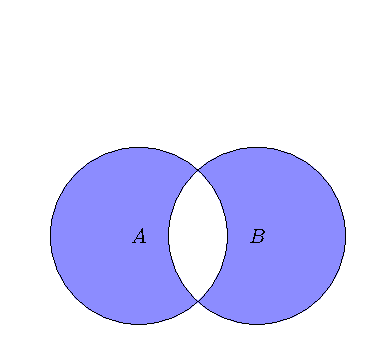
\includegraphics{grupo-boleano.pdf}
		\end{figure}

		\begin{figure}[h]
			\centering
			\caption{A associatividade \'e representada pela \'area em azul:}
			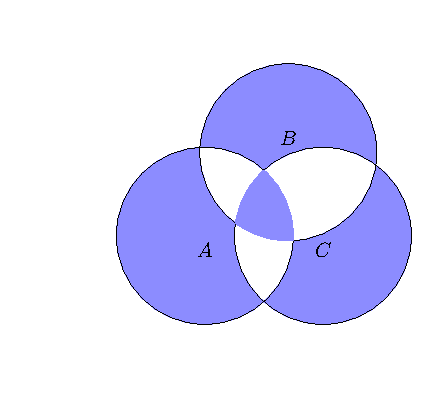
\includegraphics{grupo-boleano-associatividade.pdf}
		\end{figure}
		Assim $\mathcal{B}(X)$ \'e um grupo comutativo, o elemento neutro e $\emptyset$ e $A^{-1} = A$ pois $A + A = \emptyset$.
	\end{enumerate}
\end{exemplos}

\begin{lema}
Seja $(G,*)$ um grupo.
\begin{enumerate}[label=({\roman*})]
\item Vale a lei do cancelamento: se $x * a = x * b$ ou $a * x = b * x$, ent\~ao $a = b$.
\item O elemento neutro {\'e} {\'u}nico.
\item Existe um {\'u}nico inverso para cada $x\in G$.
\item Para todos $x$, $y\in G$ temos $(x*y)^{-1}=y^{-1}*x^{-1}$. Por indu{\c c}{\~a}o, $x_{1}$, $x_{2}$, \dots $x_{n-1}$, $x_{n}\in G$
	\[
		(x_1*x_2*...*x_{n-1}*x_n)^{-1} = x^{-1}_n*x^{-1}_{n-1}*...*x^{-1}_2*x^{-1}_1.
	\]
\item Para todo $x\in G, (x^{-1})^{-1}=x$.
\end{enumerate}
\end{lema}

\begin{definicao}
	Se $G$ \'e um grupo e se $a \in G$, defina as \textbf{pot\^encias} $a^n$, para $n \ge 1$, como sendo\index{Grupos!Pot\^encias de um elemento}
	\[
		a^1 = a\quad \mbox{e}\quad a^{n + 1} = a^na.
	\]
	Definimos $a^0 = 1$ e se $n$ \'e um inteiro positivo, definimos
	\[
		a^{-n} = (a^{-1})^n.
	\]
\end{definicao}

\begin{lema}
	Se $G$ \'e um grupo e $a$, $b \in G$, ent\~ao $(ab)^{-1} = b^{-1}a^{-1}$.
\end{lema}

\begin{lema}
	Sejam $G$ um grupo, $a$, $b \in G$ e $m$, $n \ge 1$. Ent\~ao
	\begin{align*}
		a^{m + n} = a^ma^n\\
		(a^m)^n = a^{mn}.
	\end{align*}
\end{lema}

\begin{proposicao}
	Sejam $G$ um grupo, $a$, $b \in G$ e $m$, $n \in \Z$.
	\begin{enumerate}[label=({\roman*})]
		\item Se $a$ e $b$ comutam, ent\~ao $(ab)^n = a^nb^n$.
		\item $(a^m)^n = a^{mn}$
		\item $a^ma^n = a^{m + n}$ 
	\end{enumerate}
\end{proposicao}

\begin{definicao}
	Seja $G$ um grupo e $a \in G$. Se $a^k = 1$ para algum $k \ge 1$, ent\~ao o menor expoente $k \ge 1$ \'e chamado de \textbf{ordem} de $a$. Se n\~ao existe tal pot\^encia, dizemos que $a$ tem \textbf{ordem infinita}.\index{Ordem!de elemento}
\end{definicao}

\begin{teorema}\label{ordem_elemento}
	Se $a \in G$ \'e um elemento de ordem $n$, ent\~ao $a^m = 1$ se, e somente se, $n | m$.
\end{teorema}
\begin{prova}
	Suponha que $a^m = 1$. Assim pelo Algor{\'\i}tmo da Divis\~ao de Euclides, existem inteiros $q$ e $r$ tais que
	\[
		a^m = a^{nq + r}
	\]
	onde $0 \le r \le n$. Assim
	\[
		a^r = a^ma^{-nq} = 1.
	\]
	Se $r > 0$, obtemos uma contradi\c{c}\~ao com a ordem de $a$. Logo $r = 0$ e portanto $n | m$. Agora, se $n | m$, ent\~ao
	\[
		a^m = a^{nq} = 1
	\]
	como quer{\'\i}amos.
\end{prova}

\begin{proposicao}
	Se $G$ \'e um grupo finito, ent\~ao todo $x \in G$ tem ordem finita.
\end{proposicao}
\begin{prova}
	Seja $x \in G$. Considere o conjunto $\{1, x, x^2, \dots, x^n,\dots\}$. Como $G$ \'e finito, existem inteiros $m > n$ tais que $x^m = x^n$, isto \'e, $x^{m - n} = 1$. Portanto $x$ tem ordem finita.
\end{prova}

% section definicao_e_propriedades (end)

\section{Subgrupos} % (fold)
\label{sec:subgrupos}
\begin{definicao}
	Seja $(G, \cdot)$. Um conjunto n\~ao vazio $H$ de $G$ \'e um \textbf{subgrupo}, que denotaremos por $H \le G$, quando com a opera\c{c}\~ao de $G$, o conjunto $H$ \'e um grupo, isto \'e, quando as condi\c{c}\~oes seguintes s\~ao satisfeitas:\index{Subgrupos}
	\begin{enumerate}[label=({\roman*})]
		\item $h_1h_2 \in H$ para todos $h_1$, $h_2 \in H$;
		\item $1 \in H$;
		\item Se $x \in H$, ent\~ao $x^{-1} \in H$.
	\end{enumerate}
\end{definicao}

\begin{proposicao}
	Um subconjunto $H$ de um grupo $G$ \'e um subgrupo se, e somente se, $H$ \'e n\~ao vazio e para quaisquer $x$, $y \in H$ temos $xy^{-1} \in H$.
\end{proposicao}
\begin{prova}
	A ida \'e imediata. Agora, suponha que $H$ n\~ao \'e vazio e que $xy^{-1} \in H$ para todos $x$, $y \in H$. Assim tomando $x \in H$ temos $1 = xx^{-1} \in H$. Se $y \in H$, ent\~ao $y^{-1} = 1y^{-1} \in H$ e finalmente se $x$ e $y \in H$, ent\~ao $xy = x(y^{-1})^{-1} \in H$. Portanto $H$ \'e um subgrupo de $G$.
\end{prova}

\begin{exemplos}
	\begin{enumerate}[label=({\arabic*})]
		\item Se $G$ \'e um grupo, ent\~ao $\{1\}$ e $G$ s\~ao subgrupos de $G$ chamados de \textbf{trivias}.\index{Grupos!Triviais}
		\item $(2\Z,+)$ \'e um subgrupo de $(\Z,+)$. De maneira geral, se $n$ \'e um inteiro qualquer, ent\~ao $(n\Z,+)$ \'e um subgrupo de $(\Z,+)$.
		\item O conjunto $V = \{(1), (12)(34), (13)(24), (14)(23)\}$ \'e um subgrupo de $S_4$.
		\item Seja $G$ um grupo qualquer. COnsidere o subconjunto
		\[
			Z(G) = \{x \in G \mid xg = gx\ \mbox{para todo } g \in G\}.
		\]
		Mostre que $Z(G) \le G$. Este subgrupo $Z(G)$ \'e chamado de \textbf{centro} de $G$. O grupo $G$ \'e abeliano se, e s\'o se, $Z(G) = G$.\index{Grupos!Centro}
	\end{enumerate}
\end{exemplos}

\begin{proposicao}\label{subgrupo_em_grupos_finitos}
	Um conjunto n\~ao vazio de um grupo finito $G$ \'e um subgrupo de $G$ se, e somente se, $H$ \'e fechado, isto \'e, se dados $a$ e $b \in H$, ent\~ao $ab \in H$. Em particular, um subconjunto n\~ao vazio de $S_n$ \'e um subgrupo se, e somente se, \'e fechado.
\end{proposicao}
\begin{prova}
	A ida \'e imediata. Para a volta, como $G$ \'e finito todos os seus elementos t\^em ordem finita. Dado $x \in H$, ent\~ao existe um inteiro $n$ tal que $x^n = 1$. Assim $1 \in H$, pois $H$ \'e fechado. Al\'em disso, $x^{-1} = x^{n - 1} \in H$. Finalmente, se $x$ e $y \in H$, ent\~ao $xy^{-1} = xy^{m - 1} \in H$, onde $m$ \'e um inteiro tal que $y^m = 1$. Portanto $H$ \'e um subgrupo de $G$.
\end{prova}

\begin{observacoes}
	\begin{enumerate}[label=({\arabic*})]
		\item A Proposi\c{c}\~ao \ref{subgrupo_em_grupos_finitos} pode falhar se $G$ for um grupo infinito. Por exemplo, seja $G = \Z$ o grupo aditivo dos inteiros. O conjunto $H = \N$ \'e fechado, mas n\~ao \'e um subgrupo de $\Z$.
		\item Para Galois, 1830, um grupo era simplesmente um conjunto fechado $H$ de $S_n$. Foi A. Cayley, em 1854 o primeiro a definir um grupo abstrato mencionando explicitamente a associatividade, o inverso e elemento neutro.
	\end{enumerate}
\end{observacoes}

Vamos fixar algumas nota\c{c}\~oes: se $H$ e $K$ s\~ao subconjuntos de um grupo $G$ (em particular, se $H$ e $K$ s\~ao subgrupos de $G$) definimos
\begin{align*}
	HK = \{hk \mid h \in H\, k \in K\}\\
	H^{-1} = \{h^{-1} \mid h \in H\}.
\end{align*}

Em geral $HK$ n\~ao \'e um subgrupo de $G$, mesmo quando $H$ e $K$ o s\~ao. (Apresente alguns exemplos!)

Dado um subconjunto n\~ao vazio $S$ de $G$, denotamos
\[
	\ger{S} = \{a_1\dots a_n \mid n \in \N, a_i \in S \mbox{ ou } a_i \in S^{-1}\}.
\]
Quando o conjunto $S$ for finito, digamos $S = \{a_1, \dots, a_n\}$ escreveremos
\[
	\ger{\{a_1,\dots, a_n\}} = \ger{a_1,\dots,a_n}.
\]
Quando $g \in G$ escrevemos
\[
	\ger{g} = \{\dots, g^{-2}, g^{-1}, 1, g, g^2,\dots\} = \{g^t \mid t \in \Z\}.
\]

\begin{proposicao}
	Sejam $G$ um grupo e $S$ um subconjunto n\~ao vazio de $G$. Ent\~ao o conjunto $\ger{S}$ \'e um subgrupo de $G$.
\end{proposicao}
\begin{prova}
	Como $S \ne \emptyset$, ent\~ao $1 \in \ger{S}$. Dados $x$, $y \in S$ temos
	\begin{align*}
		x = a_1a_2\dots a_m\\
		y = b_1b_2\dots b_n\\
	\end{align*}
	com $a_i$, $b_j \in S$ ou $a_i$, $b_j \in S^{-1}$ para todo $i$ e todo $j$. Logo $y^{-1} = b_n^{-1}\dots b_2^{-1}b_1^{-1}$ para todo $j$, da{\'\i}
	\[
		xy^{-1} = a_1\dots a_mb_{n}^{-1}\dots b_2^{-1}b_1^{-1} \in \ger{S}.
	\]
	Portanto $\ger{S}$ \'e um subgrupo de $G$.
\end{prova}

\begin{definicao}
	Sejam $G$ um grupo e $S$ um subconjunto n\~ao vazio de $G$. Ent\~ao $\ger{S}$ \'e chamado de \textbf{subgrupo gerado} por $S$.\index{Subgrupos!gerados por um conjunto}
\end{definicao}

\begin{definicao}
	Um grupo \'e \textbf{c{\'\i}clico} quando ele pode ser gerado por um elemnto, isto \'e, quando $G = \ger{g}$ para algum $g \in G$.\index{Grupos!C{\'\i}clicos}
\end{definicao}

\begin{definicao}
	A \textbf{ordem} de um grupo $G$ \'e o n\'umero de elementos em $G$.\index{Grupos!Ordem}
\end{definicao}

\begin{proposicao}\label{ordem_de_elemento}
	Seja $G$ um grupo finito e seja $\alpha \in G$. Ent\~ao a ordem de $\alpha$ \'e igual ao n\'umero de elementos em $\ger{\alpha}$, isto \'e,
	\[
		|\alpha| = |\ger{\alpha}|.
	\]
\end{proposicao}
\begin{prova}
	Como $G$ \'e finito, existe um menor inteiro $k \ge 1$ tal que $1$, $\alpha$, $\alpha^2$, \dots, $\alpha^{k - 1}$ s\~ao todos as pot\^encias distintas de $\alpha$, enquanto que em $1$, $\alpha$, $\alpha^2$, \dots, $\alpha^{k - 1}$, $\alpha^k$ temos repeti\c{c}\~oes de pot\^encias. Da{\'\i} $\alpha^k = \alpha^i$ para algum $0 \le i \le k - 1$. Se $i \ge 1$, ent\~ao $\alpha^{k - i} = 1$, o que contradiz a escolha de $k$. Logo $a^k = a^0 = 1$ e assim $k$ \'e a ordem de $\alpha$.

	Agora seja $H = \{1, \alpha, \alpha^2, \dots, \alpha^{k - 1}\}$. Ent\~ao $|H| = k$. Seja $\alpha^i \in \ger{\alpha}$, com $i \in \Z$. Pelo Algor{\'\i}tmo da Divis\~ao de Euclides, existem $q$, $r \in \Z$ tais que $i = qk + r$, com $0 \le r < k$. Assim $\alpha^i = \alpha^{qk}\alpha^r = \alpha^r \in H$, isto \'e, $\ger{\alpha} \sub H$. Como $H \sub \ger{\alpha}$ pela defini\c{c}\~ao de $H$, ent\~ao $H = \ger{\alpha}$. Portanto,
	\[
		|\alpha| = |\ger{\alpha}|
	\]
	como quer{\'\i}amos.
\end{prova}

\begin{teorema}
	Se $G = \ger{a}$ \'e um grupo c{\'\i}clico de ordem $n$, ent\~ao $a^k$ \'e um gerador de $G$ se, e somente se, $mdc(k,n) = 1$.
\end{teorema}
\begin{prova}
	Se $a^k$ \'e um gerador de $G$, ent\~ao $a = a^{kt}$ para algum $t \in \Z$. Da{\'\i} $a^{kt - 1} = 1$ e ent\~ao pelo Teorema \ref{ordem_elemento}, $n | (kt -1)$, isto \'e, $nu = kt - 1$ para algum $u \in \Z$. Logo, $mdc(k,n) = 1$.

	Agora, se $mdc(k,n) = 1$, ent\~ao existem $p$, $q \in \Z$ tais que $kp + nq = 1$. Da{\'\i}
	\[
		a = a^{kp + nq} = a^{nq}(a^k)^p = (a^k)^p
	\]
	e ent\~ao $G = \ger{a}$.
\end{prova}

\begin{definicao}
	O subgrupo $\ger{\{xyx^{-1}y^{-1} \mid x, y \in G\}}$ \'e o \textbf{subgrupo dos comutadores} do grupo $G$. Ele ser\'a denotado por $G'$. Note que $G$ \'e abeliano se, e somente se, $G' = \{1\}$.\index{Subgrupos!dos comutadores}
\end{definicao}


% section subgrupos (end)

\section{Teorema de Lagrange} % (fold)
\label{sec:teorema_de_lagrange}

Sejam $G$ um grupo e $H$ um subgrupo de $G$. Sobre $G$ defina a rela\c{c}\~ao $\sim_{E}$ da seguinte maneira
\[
	y \sim_{E} x \mbox{ se, e somente se, exite } h \in H \mbox{ tal que } y = xh.
\]
\'E imediato verificar que $\sim_{E}$ \'e uma rela\c{c}\~ao de equival\^encia. Dado $x \in G$ a classe de equival\^encia de $x$ \'e o conjunto
\[
	xH = \{y \in G \mid y \sim_{E} x\} = \{xh \mid h \in H\}
\]
que chamaremos de \textbf{classe lateral \`a esquerda} de $H$ em $G$. Quando n\~ao houver chance de confus\~ao, diremos simplesmente classe lateral de $x$ \`a esquerda. Observe que $y \in xH$ se, e s\'o se, $yH = xH$.\index{Grupos!classe lateral \`a esquerda}

Analogamente, podemos definir a seguinte rela\c{c}\~ao de equival\^encia:
\[
	y \sim_{D} x \mbox{ se, e somente se, exite } h \in H \mbox{ tal que } y = hx. 
\]
Obtemos assim as \textbf{classes laterais \`a direita} de $H$ em $G$. A classe lateral de $x$ \`a direita \'e dada por\index{Grupos!classe lateral \`a direita}
\[
	Hx = \{y \in G \mid y \sim_{D} x\} = \{hx \mid h \in H\}.
\]

\begin{definicao}
	Dado um grupo $G$ e $H$ um subgrupo de $G$, o conjunto das classes laterais \`a esquerda de $H$ em $G$ \'e denotado por
	\[
		\left(\dfrac{G}{H}\right)_E = \{xH \mid x \in G\}.
	\]
	Analogamente, definimos
	\[
		\left(\dfrac{G}{H}\right)_D = \{Hy \mid y \in G\}.
	\]
\end{definicao}

\begin{definicao}
	A cardinalidade do conjunto das classes laterais \`a esquerda, $(G/H)_E$, \'e o \textbf{{\'\i}ndice} de $H$ em $G$ e ser\'a denotado por $[G:H]$.\index{Grupos!{\'\i}ndice}
\end{definicao}

\begin{observacao}
	O {\'\i}ndice de $H$ em $G$ tamb\'em \'e a cardinalidade do conjunto das classes laterais \`a direita de $H$ em $G$. De fato, \'e imediato verificar que a aplica\c{c}\~ao
	\begin{align*}
		\varphi : \left(\dfrac{G}{H}\right)_E \to \left(\dfrac{G}{H}\right)_D\\
		xH \mapsto Hx^{-1}
	\end{align*}
	est\'a bem definida e \'e uma bije\c{c}\~ao.
\end{observacao}

\begin{proposicao}
	Todas as classes laterais de $H$ em $G$ t\^em a mesma cardinalidade, igual \`a cardinalidade de $H$.
\end{proposicao}
\begin{prova}
	Basta verificar que a aplica\c{c}\~ao
	\begin{align*}
		\varphi : H \to \left(\dfrac{G}{H}\right)_E\\
		x \mapsto xH
	\end{align*}
	\'e uma bije\c{c}\~ao.
\end{prova}

\begin{teorema}[Teorema de Lagrange]\label{teorema_de_lagrange}
	Sejam $G$ um grupo finito e $H$ um subgrupo de $G$. Ent\~ao
	\[
		|G| = |H|[G:H],
	\]
	em particular, a ordem e o {\'\i}ndice de $H$ dividem a ordem de $G$.
\end{teorema}
\begin{prova}
	Seja $\{a_1H, a_2H, \dots, a_tH\}$ a fam{\'\i}lia de todas as classes laterais distintas de $H$ em $G$. Ent\~ao
	\[
		G = a_1H \cup a_2H \cup \cdots \cup a_tH
	\]
	e assim
	\[
		|G| = |a_1H| + |a_2H| + \cdots + |a_tH|.
	\]
	Mas, $|H| = |a_iH|$ para todo $i = 1$, \dots, $t$, onde $t = [G:H]$. Portanto
	\[
		|G| = |H|[G:H]
	\]
	como quer{\'\i}amos.
\end{prova}

\begin{corolario}\label{primeiro_corolario_lagrange}
	Sejam $G$ um grupo finito e $\alpha \in G$. Ent\~ao a ordem de $\alpha$ divide a ordem de $G$.
\end{corolario}
\begin{prova}
	Segue da Proposi\c{c}\~ao \ref{ordem_de_elemento} pois $|\alpha| = |\ger{\alpha}|$.
\end{prova}

\begin{corolario}\label{segundo_corolario_lagrange}
	Seja $G$ um grupo. Se $K \le H \le G$ com $K \unlhd G$ e $H \unlhd G$, ent\~ao
\[
  \dfrac{G/K}{H/K} \cong \dfrac{G}{H}.
\]
\end{corolario}
\begin{prova}
	A prova \'e deixada para o leitor.
\end{prova}

\begin{corolario}
	Se $G$ \'e um grupo finito, ent\~ao $a^{|G|} = 1$ para todo $a \in G$.
\end{corolario}
\begin{prova}
	Se $a$ possui ordem, ent\~ao pelo Corol\'ario \ref{primeiro_corolario_lagrange}, devemos ter $|G| = dm$ para algum $m \ge 1$. Logo $a^{|G|} = a^{dm} = 1$.
\end{prova}

\begin{corolario}
	Se $p$ \'e um n\'umero primo, ent\~ao todo grupo $G$ de ordem $p$ \'e c{\'\i}clico.
\end{corolario}
\begin{prova}
	Se $a \in G$, $a \ne 1$, ent\~ao $a$ tem ordem $d > 1$, o que \'e imposs{\'\i}vel. Logo $G = \ger{a}$.
\end{prova}

\begin{proposicao}
	Seja $G$ um grupo abeliano.
	\begin{enumerate}[label=({\roman*})]
		\item Se $a$, $b \in G$ s\~ao dois elementos de ordem finita tais que $mdc\{|a|, |b|\} = 1$, ent\~ao $|ab| = |a||b|$.
		\item Se $r:= sup\{|g| : g \in G\}$ \'e finito, ent\~ao $|x|$ divide $r$ para cada $x \in G$.
	\end{enumerate}
\end{proposicao}
\begin{prova}
	\begin{enumerate}[label=({\roman*})]
		\item Sejam $|a| = m$, $|b| = n$ e $z = |ab|$. Como $a$ e $b$ comutam, temos $(ab)^{mn} = (a^m)^n(b^n)^m = 1$. Logo $z$ \'e um divisor de $mn$. Agora, $(ab)^z = 1$, da{\'\i} $a^z = b^{-z} \in \ger{a}\cap\ger{b}$. Mas $mdc(m,n) = 1$, logo $\ger{a}\cap\ger{b} = \{1\}$. Ent\~ao $a^z = b^z = 1$ e portanto $z$ \'e um m\'ultiplo de $m$ e de $n$. Como $m$ e $n$ s\~ao relativamente primos, $z$ \'e um m\'ultiplo de $mn$. Portanto, $z = mn$ como quer{\'\i}amos.
		\item Inicialmente vamos provas a seguinte afirma\c{c}\~ao:

		``Se $a$, $b \in G$ s\~ao dois elementos de ordem finita, ent\~ao existe $c \in G$ tal que $|c| = mmc\{|a|, |b|\}$.''

		Sejam $m = |a|$ e $n = |b|$. Se $mdc(m, n) = 1$, ent\~ao pelo item anterior podemos tomar $c = ab$. Se $mdc(m, n) \ne 1$, escreva
		\begin{align*}
			m = p_1^{\alpha_1}\cdots p_k^{\alpha_k}p_{k + 1}^{\alpha_{k + 1}}\cdots p_t^{\alpha_t}\\
			m = p_1^{\beta_1}\cdots p_k^{\beta_k}p_{k + 1}^{\beta_{k + 1}}\cdots p_t^{\beta_t}
		\end{align*}
		onde $0 \le \alpha_i < \beta_i$ para $i = 1$, \dots, $k$, $\alpha_j \ge \beta_j \ge 0$ para $j = k + 1$, \dots, $t$ e os primos $p_i$ s\~ao todos distintos.

		Considere os elementos
		\begin{align*}
			a_1 = a^{p_1^{\alpha_1}\cdots p_k^{\alpha_k}}\\
			b_1 = b^{p_{k + 1}^{\beta_{k + 1}}\cdots p_t^{\beta_t}}.
		\end{align*}
		Assim
		\begin{align*}
			|a_1| = p_{k + 1}^{\alpha_{k + 1}}\cdots p_t^{\alpha_t}\\
			|b_1| = p_1^{\beta_1}\cdots p_k^{\beta_k}.
		\end{align*}
		e ent\~ao $mdc\{|a_1|, |b_1|\} = 1$  e pelo item anterior basta tomar $c = a_1b_1$. Logo a afirma\c{c}\~ao est\'a provada.

		Para provar o item b), suponha que $r := sup\{|g| \mid g \in G\}$ \'e finito e tome $y \in G$ tal que $|y| = r$. Suponha que existe $x \in G$ tal que $|x|$ n\~ao divide $|y|$. Assim $s = mdc\{|x|, |y|\} > r$ e pela afirma\c{c}\~ao anterior existe $x \in \ger{x, y} \sub G$ tal que $|c| = s > r$, o que contradiz a defini\c{c}\~ao de $r$.
	\end{enumerate}
\end{prova}

\begin{proposicao}
	Seja $G$ um grupo e sejam $K < H < G$. Ent\~ao
	\[
		[G:K] = [G:H][H:K].
	\]
\end{proposicao}
% section teorema_de_lagrange (end)

\section{Subgrupos Normais e Grupos Quocientes} % (fold)
\label{sec:subgrupos_normais_e_grupos_quocientes}

Sejam $G$ um grupo e $H$ um subgrupo de $G$. Considere o conjunto das classes laterais \`a esquerda de $H$ em $G$:
\[
	\left(\dfrac{G}{H}\right) = \{xh \mid x \in G\}.
\]
Queremos definir uma opera\c{c}\~ao em $G/H$ de modo que este conjunto se torne um grupo. O meio natural de fazer isso \'e definindo
\begin{align}\label{operacao_no_grupo_quociente}
	(xH)\cdot (yH) = (xy)H
\end{align}
onde $x$ , $y \in G$. Como uma mesma classe lateral possui v\'arios representantes distintos, precisamos garantir que esta opera\c{c}\~ao est\'a bem definida, isto \'e, se escolhermos outros representantes das classes $xH$ e $yH$ o resultado n\~ao se altera. Para isso sejam $x$, $y \in G$ e $h$, $k \in H$. Ent\~ao $x$ e $xh$ s\~ao representantes da mesma classe $xH$, $y$ e $yH$ s\~ao representantes da mesma classe $yH$. Assim precisamos ter
\[
	xyH = xhykH,
\]
para todos $x$, $y \in G$ e para todos $y$, $k \in H$. Isto \'e, devemos ter
\begin{align*}
	y^{-1}x^{-1}xyH = y^{-1}x^{-1}xhykH\\
	H = y^{-1}hyH
\end{align*}
para todo $y \in G$ e $h \in H$. Portanto a opera\c{c}\~ao \eqref{operacao_no_grupo_quociente} est\'a bem definida em $G/H$ se, e somente se,
\[
	y^{-1}hy \in H
\]
para todo $y \in G$ e todo $h \in H$.

\begin{proposicao}\label{condicoes_subgrupo_normal}
	Seja $H$ um subgrupo de um grupo $G$. As afirma\c{c}\~oes seguintes s\~ao equivalentes:
	\begin{enumerate}[label=({\roman*})]
		\item a opera\c{c}\~ao \eqref{operacao_no_grupo_quociente} est\'a bem definida;
		\item $g^{-1}Hg \sub H$, para todo $g \in G$;
		\item $g^{-1}Hg = H$, para todo $g \in G$;
		\item $gH = Hg$, para todo $g \in G$.
	\end{enumerate}
\end{proposicao}
\begin{prova}
	$(i) \Leftrightarrow (ii)$ J\'a foi feito.

	$(iii) \Leftrightarrow (iv)$ Imediato.

	$(iii) \Rightarrow (ii)$ Imediato.

	$(ii) \Rightarrow (ii)$ Suponha que $gHG^{-1} \sub H$ para todo $g \in G$. Sejam $h \in H$ e $g \in G$. Temos
	\[
		h = g^{-1}(ghg^{-1})g \in g^{-1}(gHg^{-1})g \sub g^{-1}Hg,
	\]
	como quer{\'\i}amos.
\end{prova}

\begin{definicao}
	Um subgrupo $H$ \'e um \textbf{subgrupo normal} de $G$, e escrevemos $H \unlhd G$, se ele satisfaz as afirma\c{c}\~oes equivalentes da Proposi\c{c}\~ao \ref{condicoes_subgrupo_normal}. Neste caso, como as classes laterais \`a esquerda de $H$ s\~ao iguais \`as classes laterais \`a direita de $H$, vamos cham\'a-las simplesmente de \textbf{classes laterais} de $H$.
\end{definicao}

\begin{exemplos}
	\begin{enumerate}[label=({\arabic*})]
		\item $\{1\}$ e $G$ s\~ao subgrupos normais de $G$.
		\item $Z(G) \unlhd G$. Mais geralmente, se $H \le Z(G)$, ent\~ao $H \unlhd G$.
		\item $G' = \{xyx^{-1}y^{-1} \mid x, y \in G\}$ \'e um subgrupo normal de $G$.
		\item Se $[G:H] = 2$, ent\~ao $H \unlhd G$.
		\item Se $G$ \'e abeliano, ent\~ao todo subgrupo de $G$ \'e normal.
	\end{enumerate}
\end{exemplos}

\begin{teorema}
	Seja $G$ um grupo e seja $H$ um subgrupo normal de $G$. Ent\~ao o conjunto das classes laterais, com o opera\c{c}\~ao induzida de $G$, \'e um grupo.
\end{teorema}

\begin{definicao}
	Sejam $G$ um grupo e $H$ um subgrupo normal de $G$. O grupo de suas classes laterais, com a opera\c{c}\~ao induzida de $G$, \'e chamado de \textbf{grupo quociente} de $G$ por $H$ e ser\'a denotado por $\dfrac{G}{H}$ ou $G/H$.\index{Grupos!Quociente}
\end{definicao}

\begin{proposicao}\label{grupo_com_ordem_potencia_de_dois}
	Se $G$ \'e um grupo finito tal que para todo $g \in G$, $g^2 = 1$, ent\~ao $|G| = 2^k$ para algum $k \in \N$.
\end{proposicao}
\begin{prova}
	Como $g^2 = 1$, para todo $g \in G$, ent\~ao $G$ \'e abeliano e assim todos os seus subgrupos s\~ao normais.

	Se $|G| = 1$, nada h\'a a fazer. Suponha ent\~ao que o resultado seja v\'alido para todo grupo $G$ de ordem menor que $|G| = n > 1$. Tome $g \in G$, $g \ne 1$. Sabemos que $g^2 = 1$, assim $H = \ger{g} = \{1,g\}$ e $H$ \'e normal em $G$. Considere o grupo $(G/H,\cdot)$. Um vez que $x^2 = 1$, ent\~ao $(xH)^2 = x^2H = H$, isto \'e, para todo $xH \in G/H$, vale que $(xH)^2 = \bar{1}$. Al\'em disso,
	\[
		\left|\dfrac{G}{H}\right| = [G:H] = \dfrac{n}{2} < n.
	\]
	Logo pela hip\'otese de indu\c{c}\~ao, $|G/H| = 2^{k - 1} = n/2$. Portanto, $|G| = n = (n/2)2 = 2^k$, como quer{\'\i}amos.
\end{prova}

\begin{proposicao}\label{construcao_grupo_dihedral}
	Se $G$ \'e um grupo com $|G| = 2p$, $p$ primo {\'\i}mpar, ent\~ao
	\[
		G = \{1, a, b, b^2, \dots, b^{p - 1}, ab, ab^2, \dots, ab^{p - 1}\}
	\]
	onde $|a| = 2$, $|b| = p$ e $ab = b^ia$ com $i = 1$ ou $i = p - 1$.
\end{proposicao}
\begin{prova}
	Como $|G| = 2p$, que \'e par, existe $a \in G$, $a \ne 1$ tal que $a^2 = 1$, isto \'e, $a = a^{-1}$. Agora, pela Proposi\c{c}\~ao \ref{grupo_com_ordem_potencia_de_dois}, existe $c \in G$ tal que $|c| = p$ ou $|c| = 2p$. Se $|c| = 2p$, ent\~ao $|c^2| = p$. Logo existe $b \in G$ tal que $|b| = p$. Seja $H = \ger{b}$. Como $[G:H] = 2$, ent\~ao $H \unlhd G$. Assim para $a \in G$ e $b \in H$ temos $aba^{-1} \in H$. Consequentemente, existe $1 \le i \le p - 1$ tal que $aba^{-1} = b^i$. \'E f\'acil verificar que $(aba^{-1})^n = b^{ni}$ para todo $n$. Ent\~ao como $|a| = 2$
	\[
		b^{i^2} = (aba^{-1})^i = ab^ia^{-1} = b,
	\]
	ou seja, $b^{i^2} - 1 = 1$. Mas $|b| = p$, da{\'\i} $p | (i^2 - 1)$. Logo $p | (i - 1)$ ou $p | (i + 1)$. Como $1 \le i \le p - 1$, ent\~ao $i = 1$ ou $i = p - 1$.

	Agora, $[G:H] = 2$, ent\~ao $G = H \cup aH$ pois $|a| = 2$, $|b| = p$ e $p$ \'e um primo {\'\i}mpar. Portanto,
	\[
		G = \{1, a, b, b^2, \dots, b^{p - 1}, ab, ab^2, \dots, ab^{p - 1}\}	
	\]
	onde $ab = b^ia$ com $i = 1$ ou $i = p - 1$.
\end{prova}

\begin{observacao}
	No caso em que $i = 1$, obtemos um grupo abeliano c{\'\i}clico de ordem $2p$. E no caso em que $i = p - 1$, temos um grupo n\~ao abeliano chamado \textbf{grupo dihedral} de ordem $2p$.\index{Grupos!Dihedral}
\end{observacao}

\begin{notacao}
	No caso geral, o grupo $G$ da Proposi\c{c}\~ao \ref{construcao_grupo_dihedral} ser\'a denotado por
	\begin{align}\label{grupo_dihedral}
		D_{2n} = \ger{a,b \mid a^2 = b^n = 1, ab = b^{n - 1}a} = \{1,a,b,\dots, b^{n - 1}, ab, \dots, ab^{n - 1}\}.
	\end{align}
	E \'e chamado de \textbf{grupo dihedral} de ordem $2n$. Em alguns casos, utiliza-se tamb\'em a nota\c{c}\~ao $D_n$ para o grupo \eqref{grupo_dihedral}
\end{notacao}

\begin{proposicao}
	Sejam $G$ um grupo e $G'$ seu subgrupo dos comutadores. Ent\~ao,
	\begin{enumerate}[label=({\roman*})]
		\item $G/G'$ \'e abeliano.
		\item $G'$ \'e o menor subgrupo normal de $G$ com esta propriedade, isto \'e, se $H \unlhd G$ \'e tal que $G/H$ \'e abeliano, ent\~ao $G'\sub H$.
	\end{enumerate}
\end{proposicao}


\begin{proposicao}
	Sejam $G$ um grupo e $Z(G)$ seu centro. Se o quociente $G/Z(G)$ \'e c{\'\i}clico, ent\~ao $G = Z(G)$. Em particular, o {\'\i}ndice de $Z(G)$ em $G$ nunca \'e igual a um n\'umero primo.
\end{proposicao}
\begin{prova}
	Seja $\overline{z}$ um gerador de $G/Z(G)$. Dado $g \in G$, existe $i \in \Z$ tal que $\overline{g} = \overline{z}^i$. Logo $g = z^ih$ para algum $h \in Z(G)$. Sejam $g_1$, $g_2 \in G$, com $g_1 = z^ih_1$ e $g_2 = z^jh_2$, para alguns $i$, $j \in \Z$ e $h_1$, $h_2 \in H$. Assim
	\[
		g_1g_2 = z^ih_1z^jh_2 = z^{i+j}h_1h_2 = z^jh_2z^ih_1 = g_2g_1.
	\]
	Portanto $G$ \'e abeliano, isto \'e, $G = Z(G)$
\end{prova}

% section subgrupos_normais_e_grupos_quocientes (end)

\section{Homomorfismo de Grupos} % (fold)
\label{sec:homomorfismo_de_grupos}

\begin{definicao}
	Se $(G,\cdot)$ e $(H,*)$ s\~ao grupos, ent\~ao a aplica\c{c}\~ao $\phi : G \to H$ \'e um \textbf{homomorfismo de grupos} se\index{Homomorfismo}
	\begin{align}\label{definicao_homomorfismo}
		\phi(x\cdot y) = \phi(x)*\phi(y)
	\end{align}
	para todos $x$, $y \in G$. Se $\phi$ tamb\'em \'e uma bije\c{c}\~ao, ent\~ao $\phi$ \'e chamada de um \textbf{isomorfismo}. Os grupos $G$ e $H$ s\~ao chamados de \textbf{isomorfos} e escrevemos $G \cong H$, se existe um isomorfismo $\phi: G \to H$.\index{Homomorfismo!Isomorfismo}
\end{definicao}

\begin{exemplos}
	\begin{enumerate}[label=({\arabic*})]
		\item $Id : G \to G$ tal que $Id(g) = g$ \'e o homomorfismo \textbf{identidade}.
		\item $e : G \to H$ tal que $e(g) = 1_H$ \'e o homomorfismo \textbf{trivial}.
		\item Seja $n \in \Z$ fixo. Ent\~ao $\phi_n : (\Z,+) \to (\Z, +)$ tal que $\phi_n(z) = nz$ \'e um homomorfismo. De modo geral, se $G$ \'e um grupo abeliano, ent\~ao $\phi_n : (G, \cdot) \to (G, \cdot)$ tal que $\phi_n(g) = g^n$ \'e um homomorfismo.
		\item Seja $H \unlhd G$, ent\~ao $\pi : G \to G/H$ tal que $\pi(g) = gH$ \'e um homomorfismo chamado de \textbf{proje\c{c}\~ao can\^onica}.\index{Homomorfismo!Proje\c{c}\~ao Can\^onica}
		\item Seja $g \in G$ fixo. Ent\~ao $\phi_g : G \to G$ tal que $\phi_g(x) = gxg^{-1}$ \'e um isomorfismo.
	\end{enumerate}
\end{exemplos}

\begin{lema}
	Seja $\phi : G \to H$ um homomorfismo de grupos.
	\begin{enumerate}[label=({\roman*})]
		\item $\phi(1_G) = 1_H$
		\item $\phi(g^{-1}) = (\phi(g))^{-1}$
		\item $\phi(g^n) = (\phi(g))^n$ para todo $n \in \Z$.
	\end{enumerate}
\end{lema}
\begin{prova}
	Exerc{\'\i}cio.
\end{prova}

\begin{lema}
	Sejam $G$ e $H$ grupos e $\phi : G \to H$ um homomorfismo. Ent\~ao:
	\begin{enumerate}[label=({\roman*})]
		\item O conjunto $\ker\phi = \{x \in G \mid \phi(x) = 1_H\}$ \'e um subgrupo normal de $G$ chamado de \textbf{n\'ucleo} ou \textbf{kernel} de $\phi$.\index{Homorfismo!Kernel}

		\item O conjunto $\im\phi = \{y \in H \mid y = \phi(x) \mbox{ para algum } x \in G\}$ \'e um subgrupo de $H$ chamado de \textbf{imagem} de $\phi.$\index{Homomorfismo!Imagem}

		\item Sejam $\phi : (G, \cdot) \to (H, *)$ e $\psi : (H,*) \to (\mathcal{G},\times)$ dois homomorfismos de grupos. Ent\~ao a composi\c{c}\~ao $\psi\circ\phi : (G, \cdot) \to (\mathcal{G}, \times)$ \'e um homomorfismo.
	\end{enumerate}
\end{lema}
\begin{prova}
	Exerc{\'\i}cio.
\end{prova}

\begin{lema}\label{imagem_direta_e_inversa_de_subgrupos}
	Seja $\phi : G \to H$ um homomorfismo de grupos.
	\begin{enumerate}[label=({\roman*})]
		\item Se $P \le G$, ent\~ao $\phi(P) \le H$ e $\phi^{-1}(\phi(P)) = P\ker\phi$.

		\item Se $R \le H$, ent\~ao $\phi^{-1}(R)$ \'e um subgrupo de $G$ contendo $\ker\phi$ e $\phi(\phi^{-1}(R)) = R \cap \im\phi$.
	\end{enumerate}
\end{lema}
\begin{prova}
	\begin{enumerate}[label=({\roman*})]
		\item A prova de que $\phi(P)$ \'e um subgrupo de $H$ \'e deixada para o leitor. Provemos que $\phi^{-1}(\phi(P)) = P\ker\phi$. Seja $xk \in P$. Temos
		\[
			\phi(xk) = \phi(x)\phi(k) = \phi(x) \in \phi(P)
		\]
		da{\'\i} $P\ker\phi \sub \phi^{-1}(\phi(P))$. Agora, seja $y \in \phi^{-1}(\phi(P))$. Por defini\c{c}\~ao, $\phi(y) \in \phi(P)$ e assim existe $x \in P$ tal que $\phi(x) = \phi(y)$. Isto \'e, $\phi(x^{-1}y) = 1_H$, donde $x^{-1}y \in \ker\phi$. Logo $y = x(x^{-1}y)\in P\ker\phi$. Portanto, $\phi^{-1}\phi(P) = P\ker\phi$.

		\item Como $R \le H$, ent\~ao $1_H \in R$ e como $\phi(x) = 1_H$ para todo $x \in \ker\phi$, ent\~ao $\ker\phi \sub \phi^{-1}(R)$. Fica a cargo do leitor provar que $\phi^{-1}(R)$ \'e um subgrupo de $G$. Provemos que $\phi(\phi^{-1}(R)) = R \cap \im\phi$.

		A inclus\~ao $\phi(\phi^{-1}(R)) \sub R \cap \im\phi$ \'e imediata. Agora, seja $y \in R \cap \im\phi$. Assim existe $x \in G$ tal que $\phi(x) = y$. Mas $y \in R$, da{\'\i} $x \in \phi^{-1}(R)$ e ent\~ao $y = \phi(x) \in \phi(\phi^{-1}(R))$. Portanto, $\phi(\phi^{-1}(R)) = R \cap \im\phi$.
	\end{enumerate}
\end{prova}

\begin{exemplos}
	\begin{enumerate}[label=({\arabic*})]
		\item O grupo dihedral $D_6$ \'e dado por
		\[
			D_6 = \ger{a,b \mid a^2 = b^3 = 1,\ ab = b^2a}.
		\]
		Agora, $S_3 = \{id,\alpha,\beta,\beta^2,\alpha\beta,\alpha\beta^2\}$ onde
		\[
			\alpha = \begin{pmatrix}
				1 & 2 & 3\\
				2 & 1 & 3
			\end{pmatrix},\quad
			\beta = \begin{pmatrix}
				1 & 2 & 3\\
				2 & 3 & 1
			\end{pmatrix},\quad
			id = \begin{pmatrix}
				1 & 2 & 3\\
				1 & 2 & 3
			\end{pmatrix}.
		\]
		A aplica\c{c}\~ao $\phi : S_3 \to D_6$ tal que
		\begin{align*}
			\phi(id) &= 1\\
			\phi(\alpha) &= a\\
			\phi(\beta) &= b\\
			\phi(\alpha\beta) &= ab\\
			\phi(\alpha\beta^2) &= ab^2
		\end{align*}
		\'e um homomorfismo bijetor. Portanto $S_3 \cong D_6$.

		\item Seja $G = \ger{a} = \{\dots, a^{-1}, 1, a, a^2, \dots\}$ um grupo c{\'\i}clico infinito. \'E f\'acil verificar que $\phi: (\Z, +) \to (G, \cdot)$ dada por $\phi(t) = a^t$ \'e um isomorfismo. Portanto $\Z \cong G$.
	\end{enumerate}
\end{exemplos}

\begin{teorema}[Teorema do Isomorfismo]\label{teorema_isomorfismo}
	Seja $\phi : (G, \cdot) \to (H, *)$ um homomorfismo de grupos.
	\begin{enumerate}[label=({\roman*})]
		\item A fun\c{c}\~ao
		\begin{align*}
			\overline{\phi} : \dfrac{G}{\ker\phi} \to \phi(G)\\
			a\ker\phi \mapsto \phi(a)
		\end{align*}
		\'e um isomorfismo.

		\item As seguintes fun\c{c}\~oes
		\begin{align*}
			\{\mbox{subgrupos de } G \mbox{ que cont\^em } \ker\phi\} &\longleftrightarrow \{\mbox{subgrupos de } \phi(G)\}\\
			P\quad &\xmapsto{\quad\psi\quad} \phi(P)\\
			\phi^{-1}(R)\quad &\xmapsfrom{\quad\sigma\quad} R
		\end{align*}
		s\~ao bije\c{c}\~oes, inversas uma da outra. Al\'em disso, estas bije\c{c}\~oes levam subgrupos normais em subgrupos normais, isto \'e,
		\begin{enumerate}[label=({\alph*})]
			\item Se $P \unlhd G$, ent\~ao $\phi(P) \unlhd \phi(G)$.

			\item Se $R \unlhd \phi(G)$, ent\~ao $\phi^{-1}(R) \unlhd G$.
		\end{enumerate}
	\end{enumerate}
\end{teorema}
\begin{prova}
	\begin{enumerate}[label=({\roman*})]
		\item Inicialmente precisamos verificar que $\overline{\phi}$ est\'a bem definida. Para isso sejam $a_1\ker\phi = a_2\ker\phi$. Assim $a_1 = a_2k$, onde $k \in \ker\phi$. Ent\~ao
		\[
			\phi(a_1) = \phi(a_2k) = \phi(a_2),
		\]
		logo $\overline{\phi}(a_1\ker\phi) = \overline{\phi}(a_2\ker\phi)$ e ent\~ao $\overline{\phi}$ est\'a bem definida. Al\'em disso, da defini\c{c}\~ao de $\overline{\phi}$ vemos que esta aplica\c{c}\~ao \'e sobrejetora.

		Agora, sejam $a_1\ker\phi$, $a_2\ker\phi \in \ker\phi$. Ent\~ao
		\[
			\overline{\phi}((a_1\ker\phi)(a_2\ker\phi)) = \overline{\phi}((a_1a_2)\ker\phi) = \phi(a_1a_2) = \phi(a_1)\phi(a_2) = \overline{\phi}(a_1\ker\phi)\overline{\phi}(a_2\ker\phi)
		\]
		e da{\'\i} $\overline{\phi}$ \'e um homomorfismo. Finalmente, se $a\ker\phi \in \ker\overline{\phi}$ ent\~ao
		\[
			\overline{\phi}(a\ker\phi) = \overline{\phi}(1_G\ker\phi)
		\]
		da{\'\i} $\phi(g) = \phi(1_G) = 1_H$, ou seja, $g \in \ker\phi$. Portanto $\ker\overline{\phi} = \{\ker\phi\}$ e ent\~ao $\overline{\phi}$ \'e injetora. Portanto $\overline{\phi}$ \'e um isomorfismo de grupos. Logo
		\[
			\dfrac{G}{\ker\phi} \cong \phi(G).
		\]

		\item Pelo Lema \ref{imagem_direta_e_inversa_de_subgrupos} sabemos que $\phi^{-1}(\phi(P)) = P\ker\phi$ para todo $P \le G$ e que $\phi(\phi^{-1}(R)) = R \cap \phi(G)$ para todo $R \le H$. Assim se $\ker\phi \sub P$, ent\~ao $\phi^{-1}(\phi(P)) = P$ e se $R \le \phi(G)$, ent\~ao $\phi(\phi^{-1}(R)) = R$. Logo as fun\c{c}\~oes $\psi$ e $\sigma$ s\~ao inversas uma da outra, isto \'e, s\~ao bije\c{c}\~oes.

		Agora falta provar os demais itens:
		\begin{enumerate}[label=({\alph*})]
			\item Sejam $a \in \phi(P)$ e $b \in \phi(G)$. Ent\~ao existem $x \in P$ e $y \in G$ tais que $\phi(x) = a$ e $\phi(y) = b$. Queremos mostrar que $b^{-1}ab \in \phi(P)$. De fato,
			\[
				b^{-1}ab = \phi(y^{-1})\phi(x)\phi(y) = \phi(y^{-1}xy) \in \phi(P)
			\]
			pois $P \unlhd G$. Portanto, $\phi(P) \unlhd \phi(G)$.

			\item Dados $a \in G$ e $x \in \phi^{-1}(R)$, queremos mostrar que $a^{-1}xa \in \phi^{-1}(R)$. Temos
			\[
				\phi(a^{-1}xa) = \phi(a)^{-1}\phi(x)\phi(a) \in R
			\]
			pois $R \unlhd \phi(G)$. Logo $a^{-1}xa \in \phi^{-1}(R)$, isto \'e, $\phi^{-1}(R) \unlhd G$, como quer{\'\i}amos.
		\end{enumerate}
	\end{enumerate}
\end{prova}

\begin{corolario}
	Seja $\phi : G \to H$ um homomorfismo de grupos e seja $K \le G$. Ent\~ao a fun\c{c}\~ao
	\begin{align*}
		\psi : \dfrac{K}{K \cap \ker\phi} \to \phi(K)\\
		a(K \cap \ker\phi) \mapsto \phi(a)
	\end{align*}
	\'e um isomorfismo.
\end{corolario}
\begin{prova}
	Considere o hommorfismo $\phi$ restrito a $K$;
	\begin{align*}
		\psi \coloneqq \phi|_{K} : K \to H\\
		h \mapsto \phi(h).
	\end{align*}
	\'E imediato verificar que $\psi(K) = \phi(K)$ e que $\ker\psi = \ker\phi$. Logo pelo Teorema do Isomorfismo, Teorema \ref{teorema_isomorfismo}, temos $K/\ker\psi \cong \psi(K)$, isto \'e,
	\[
		\dfrac{K}{K \cap \ker\phi} \cong \phi(K).
	\]
\end{prova}

\begin{corolario}
	Seja $H$ um subgrupo normal de $G$. Ent\~ao a fun\c{c}\~ao
	\[
		\{\mbox{subgrupos (normais) de } G \mbox{ que cont\^em } H\} \longleftrightarrow \{\mbox{subgrupos (normais) de } G/H\}.
	\]
	\'e uma bije\c{c}\~ao.
\end{corolario}
\begin{prova}
	\'E f\'acil verificar que $\phi : G \to G/H$ dada por $\phi(a) = aH$ \'e um homomorfismo sobrejetivo. Aplicando a segunda parte do Teorema do Isomorfismo, Teorema \ref{teorema_isomorfismo}, obtemos o resultado.
\end{prova}

\begin{teorema}[Teorema da Representa\c{c}\~ao]\label{teorema_da_representacao}
	Seja $G$ um grupo e $H$ um subgrupo de $G$ tal que $[G : H] = n$. Ent\~ao existe $N \sub H$, com $N \unlhd G$ tal que $G/N$ \'e um grupo isomorfo a um subgrupo de $S_n$. Mais ainda, $N$ \'e o ``maior'' subgrupo normal de $G$ que est\'a contido em $H$.
\end{teorema}
\begin{prova}
	Seja $S = G/H = \{Hx_1, \dots, Hx_n\}$ e $\mathcal{P}(S)$ o grupo das permuta\c{c}\~oes do conjunto $S$. \'E claro que $\mathcal{P}(S) \cong S_n$.

	Considere a seguinte aplica\c{c}\~ao
	\begin{align*}
		\psi : G \to \mathcal{P}(S)\\
		a \mapsto \psi_a
	\end{align*}
	onde $\psi_a : S \to S$ \'e tal que $\psi_a(Hx_i) = Hx_ia^{-1}$.

	Inicialmente para $a \in G$ temos $\psi_a(Hx_i) = \psi_a(Hx_j)$ se, e s\'o se, $Hx_ia^{-1} = Hx_ja^{-1}$. Isto \'e, $Hx_i = Hx_j$, logo $\psi_a$ \'e injetora. Como $|S| = n$, ent\~ao $\psi_a$ \'e sobrejetiva e da{\'\i} $\psi_a \in \mathcal{P}(S)$. Logo $\psi_a \in \mathcal{P}(S)$ para todo $a \in G$.

	Verifiquemos agora que $\psi$ \'e um homomorfismo de grupos. Dados $a$, $b \in G$ queremos mostrar que $\psi(ab) = \psi(a)\psi(b)$. Mas $\psi(ab) = \psi_{ab}$. Seja $Hx_i \in S$. Temos
	\[
		\psi_{ab}(Hx_i) = Hx_i(ab)^{-1} = (Hx_ib^{-1})a^{-1} = \psi_a(\psi_b(Hx_i)) = (\psi_a\circ\psi_b)(Hx_i).
	\]
	Portanto $\psi$ \'e um homomorfismo de grupos.

	Agora,
	\[
		\ker\psi = \{a \in G \mid \psi(a) = Id_S\} = \{a \in G \mid Hx_ia^{-1} = Hx_i, i = 1, \dots, n\}.
	\]
	Da{\'\i} $a \in \ker\psi$ se, e s\'o se, $Hx_ia^{-1} = Hx_i$ para todo $i = 1$, \dots, $n$. Mas isso ocorre se, e s\'o se, $Hx_i = Hx_ia$ para todo $i = 1$, \dots, $n$. Logo $a \in \ker\psi$ se, e s\'o se, $H = Hx_iax_i^{-1}$ para todo $i = 1$, \dots, $n$. Da{\'\i} $a \in \ker\psi$ se, e s\'o se, $x_iax_i^{-1} \in H$ para todo $i = 1$, \dots, $n$ e ent\~ao $a \in \ker\psi$ se, e s\'o se, $a \in x_i^{-1}Hx_i$ para todo $i = 1$, \dots, $n$. Mas $G = Hx_1 \cup \cdots \cup Hx_n$, uma uni\~ao disjunta e como $(hx_i)^{-1}H(hx_i) = x_i^{-1}Hx_i$ para todo $h \in H$, ent\~ao $a \in \ker\psi$ se, e s\'o se, $a \in x^{-1}Hx$ para todo $x \in G$. Ou seja, $a \in \ker\psi$ se, e somente se, $a \in \cap_{x \in G}(x^{-1}Hx)$. Portanto $\ker\psi = \cap_{x \in G}(x^{-1}Hx)$.

	Seja $N = \ker\psi$. Ent\~ao $N \unlhd G$ e $N \sub H$. Agora, seja $L \unlhd G$ tal que $L \sub H$. Ent\~ao $x^{-1}Lx = L \sub x^{-1}Hx$ para todo $x \in G$. Assim, $L \sub N = \cap_{x \in G}(x^{-1}Hx)$. Portanto $N$ \'e o ``maior'' subgrupo normal de $G$ contido em $H$.

	Finalmente pelo Teorema do Isomorfismo, Teorema \ref{teorema_isomorfismo}, temos
	\[
		\dfrac{G}{\ker\psi} = \dfrac{G}{N} \cong \psi(G) \le \mathcal{P}(S) \cong S_n,
	\]
	como quer{\'\i}amos.
\end{prova}

\begin{corolario}[Teorema de Cayley]\label{teorema_de_cayley}
	Se $G$ \'e um grupo de ordem $n$, ent\~ao $G$ \'e isomorfo a um subgrupo de $S_n$.
\end{corolario}
\begin{prova}
	Basta tomar $H = \{1\}$ no Teorema da Representa\c{c}\~ao, Teorema \ref{teorema_da_representacao}.
\end{prova}

% section homomorfismo_de_grupos (end)

\section{Classes de Conjuga\c{c}\~ao} % (fold)
\label{sec:classes_de_conjugacao}

Seja $G$ um grupo. Dados $x$, $y \in G$ defina
\[
	x \sim_G y \mbox{ se, e somente se, existe } a \in G \mbox{ tal que } y = a^{-1}xa.
\]

\begin{proposicao}
	Seja $G$ um grupo. A rela\c{c}\~ao $\sim_G$ define uma rela\c{c}\~ao de equival\^encia em $G$.
\end{proposicao}
\begin{prova}
	A prova \'e deixada para o leitor.
\end{prova}

\begin{definicao}
	Se $x \sim_G y$, dizemos que $x$ e $y$ s\~ao elementos \textbf{conjugados} em $G$.\index{Elementos!Conjugados}
\end{definicao}

Denote $a^{-1}xa = x^a$, onde $x$ e $a \in G$. As seguintes propriedades s\~ao v\'alidas:
\begin{enumerate}[label=({\arabic*})]
	\item $x^{1_G} = x$ para todo $x \in G$.

	\item Se $y = x^a$, ent\~ao $x = y^{a^{-1}}$ para todos $x$, $y$ e $a \in G$.

	\item $(x^a)^b = x^{ab}$ para todos $x$, $a$ e $b \in G$.
\end{enumerate}

A classe de equival\^encia de $x$ \'e dada por
\[
	C_x = \{y \in G \mid x \sim_G y\} = \{x^a \mid a \in G\}
\]
e \'e chamada de \textbf{classe de conjuga\c{c}\~ao} de $x$ em $G$.\index{Classe de Conjuga\c{c}\~ao}

Se $G$ \'e um grupo finito e existem $n$ classes de conjuga\c{c}\~ao com representantes $x_1$, $x_2$, \dots, $x_n$ ent\~ao
\[
	G = C_{x_1} \cup C_{x_2} \cup \cdots \cup C_{x_n}
\]
uma uni\~ao disjunta. Assim
\[
	|G| = |C_{x_1}| + |C_{x_2}| + \cdots + |C_{x_n}|.
\]
Observe que $C_x = \{x\}$ se, e somente se, $x \in Z(G)$ e da{\'\i} a equa\c{c}\~ao anterior pode ser escrita como
\begin{equation}\label{equacao_de_classes}
	|G| = |Z(G)| + \sum_{x \notin Z(G)}|C_x|.
\end{equation}

A equa\c{c}\~ao \eqref{equacao_de_classes} \'e chamada de \textbf{equa\c{c}\~ao de classes}.\index{Equa\c{c}\~ao de Classes}

\begin{proposicao}
	Seja $G$ um grupo e $x \in G$. Ent\~ao o conjunto $C_G(x) = \{a \in G \mid ax = xa\}$ \'e um subgrupo de $G$.
\end{proposicao}
\begin{prova}
	A cargo do leitor.
\end{prova}

\begin{proposicao}\label{ordem_da_classe_de_conjugacao}
	Seja $G$ um grupo finito e $x \in G$. Ent\~ao
	\[
		[G : C_G(x)] = |C_x|.
	\]
	Em particular, $|C_x|$ \'e um divisor de $|G|$ para todo $x \in G$.
\end{proposicao}
\begin{prova}
	Sejam $H = C_G(x)$ e $G/H = \{Ha \mid a \in G\}$ o conjunto de todas as classes laterais \`a direita de $H$ em $G$. Pelo Teorema de Lagrange, Teorema \ref{teorema_de_lagrange}, $|G| = [G : H]|H|$. Agora, considere a aplica\c{c}\~ao
	\begin{align*}
		\phi : \dfrac{G}{H} \to C_x\\
		Ha \mapsto x^a.
	\end{align*}
	Claramente $\phi$ \'e sobrejetora. Sejam $Ha$, $Hb \in G/H$ tais que $\phi(Ha) = \phi(Hb)$. Da{\'\i} $x^a = x^b$ e ent\~ao $x^{ab^{-1}} = 1$, isto \'e, $ab^{-1} \in C_G(x) = H$ e portanto $Ha = Hb$. Logo $\phi$ \'e injetiva. Assim
	\[
		|C_x| = [G : C_G(x)]
	\]
	como quer{\'\i}amos.
\end{prova}

\begin{definicao}
	Seja $p$ um n\'umero primo e $G$ um grupo. Se $|G| = p^n$, $n \in \N$, dizemos que $G$ \'e um $p$-\textbf{grupo}.\index{Grupos!$p$-grupos}
\end{definicao}

\begin{exemplos}
	\begin{enumerate}[label=({\arabic*})]
		\item Os grupos $D_8$, $\Z_8$, $\Z_4\times \Z_2$ e $\Z_2\times\Z_2\times\Z_2$ s\~ao 2-grupos de ordem $2^3$.

		\item O grupo $(\Z_{p^n}, \otimes)$ \'e um $p$-grupo de ordem $p^n$.

		\item $\Z_2\times\Z_2\times\Z_2\times\cdots$ \'e um 2-grupo infinito.
	\end{enumerate}
\end{exemplos}

\begin{observacao}
	Pelo Teorema de Lagrange, Teorema \ref{teorema_de_lagrange}, todo subgrupo de um $p$-grupo tamb\'em \'e um $p$-grupo.
\end{observacao}

\begin{teorema}
	Se $G$ \'e um $p$-grupo e $|G| = p^n > 1$, ent\~ao $|Z(G)| = p^m > 1$.
\end{teorema}
\begin{prova}
	Pela Equa\c{c}\~ao de classes, \eqref{equacao_de_classes}, obtemos
	\[
		|Z(G)| = |G| - \sum_{x \notin Z(G)}|C_x|.
	\]
	Mas para todo $x \notin Z(G)$, temos $|C_x| > 1$ e como $|C_x|$ divide $|G|$, ent\~ao $|C_x| = p^{\alpha_x}$ para todo $x \notin Z(G)$. Como $|G| = p^n > 1$, ent\~ao devemos ter $|Z(G)| = p^m > 1$.
\end{prova}

\begin{corolario}
	Se $p$ \'e um n\'umero primo e $|G| = p^2$, ent\~ao $G$ \'e um grupo abeliano.
\end{corolario}

\begin{teorema}[Teorema de Cauchy]
	Seja $p$ um divisor primo da ordem de um grupo finito $G$. Ent\~ao existe $a \in G$ tal que $|a| = p$.
\end{teorema}
\begin{prova}
	Vamos usar indu\c{c}\~ao sobre a ordem de $G$. Se $|G| = 1$, nada h\'a a fazer. Vamos supor que o teorema \'e v\'alido para todo grupo $H$ tal que $1 \le |H| < |G|$. Temos tr\^es casos para analizar.
	
	\noindent \textit{Caso 1:} $G$ \'e c{\'\i}clico.

	Seja $G = \ger{x}$  e seja $p$ um divisor primo de $|G|$. Neste caso $|x| = p^{\alpha k}$, onde $\alpha \ge 1$. Tome $a = x^{p^{\alpha - 1}k}$. Ent\~ao $a^p = 1$ e nenhum outra pot\^encia $r$ de $a$ menor que $p$ \'e tal que $a^r = 1$. Portanto $|a| = p$ como quer{\'\i}amos.

	\noindent \textit{Caso 2:} $G$ \'e abeliano e n\~ao c{\'\i}clico.

	Seja $p$ um divisor primo de $|G|$ e seja $x \in G$, $x \ne 1$. Se $p$ divide $|x|$ ent\~ao pelo \textit{Caso 1}, existe $a \in \ger{x}$ tal que $|a| = p$ e assim o teorema est\'a provado.

	Suponha ent\~ao que $p$ n\~ao divide $|x|$. Seja $N = \ger{x}$. Como $G$ \'e abeliano, ent\~ao $L = G/N$ \'e um grupo tal que $p$ divide $|L| = [G : N]$. Mas $1 \le |L| < |G|$, assim pela hip\'otese de indu\c{c}\~ao existe $\overline{b} \in L$ tal que $\overline{b} \ne \overline{1}$ e $|\overline{b}| = p$. Assim $b \notin N$ e $b^p \in N$. Seja $|N| = r$, ent\~ao $(b^p)^r = 1$ e portanto $p$ divide $|b|$. Logo pelo \textit{Caso 1}, existe $a \in \ger{b}$ tal que $|a| = p$ e ent\~ao o teorema est\'a provado.

	\noindent \textit{Caso 3:} $G$ n\~ao abeliano

	Neste caso $Z(G) \ne G$. Se $p$ divide $|Z(G)|$, ent\~ao basta usar o \textit{Caso 2}. Assim suponha que $p$ n\~ao divide $|Z(G)|$. Temos
	\[
		|G| = |Z(G)| + \sum_{x \notin Z(G)}[G : C_G(x)].
	\]
	Como $p$ divide $|G|$ ent\~ao existe $x \notin Z(G)$ tal que $p$ n\~ao divide $[G : C_G(x)]$. Portanto $p$ divide $|H|$ onde $H = C_G(x) \ne G$. Como $1 \le |H| < |G|$, ent\~ao pela hip\'otese de indu\c{c}\~ao, existe $a \in H$ tal que $|a| = p$.

	Portanto o teorema est\'a provado.
\end{prova}

% section classes_de_conjugacao (end)


\section{Grupos C{\'\i}clicos} % (fold)
\label{sec:grupos_ciclicos}

\begin{proposicao}
	\begin{enumerate}[label=({\roman*})]
		\item Se $H \sub \Z$, ent\~ao $H$ \'e um subgrupo de $(\Z, +)$ se, e somente se, $H = n\Z$ para algum $n \in \N$.
		
		\item $n\Z \sub m\Z$ se, e somente se, $m | n$. Neste caso temos $[m\Z : n\Z] = \frac{n}{m}$.
	\end{enumerate}
\end{proposicao}
\begin{prova}
	\begin{enumerate}[label=({\roman*})]
		\item Se $H = n\Z$, com $n \in \N$, ent\~ao \'e f\'acil verificar que $H \le \Z$.

		Agora seja $H \le \Z$, $H \ne \{0\}$. Tome $n = \min\{x \in H \mid x > 0\}$. Como $n \in H$ e como $H \le \Z$, ent\~ao $n\Z \sub H$. Dado $a \in H$, existem $q$ e $r \in \Z$ tais que $a = qn + r$ com $0 \le r < n$. Mas $a$, $n \in H$ da{\'\i} $r \in H$ e ent\~ao pela minimalidade de $n$ devemos ter $r = 0$. Logo $a \in n\Z$ e portanto $H = n\Z$.

		\item \'E imediato verificar que $n\Z \sub m\Z$ se, e somente se, $m | n$. Suponha que $n\Z \le m\Z \le \Z$. Assim pelo Corol\'ario \ref{segundo_corolario_lagrange} temos
		\[
			\dfrac{\Z/n\Z}{m\Z/n\Z} \cong \dfrac{\Z}{m\Z},
		\]
		da{\'\i}
		\[
			\left|\dfrac{\Z/n\Z}{m\Z/n\Z}\right| = \left|\dfrac{\Z}{m\Z}\right|.
		\]
		Ent\~ao
		\[
			\dfrac{n}{[m\Z : n\Z]} = m
		\]
		e portanto $[m\Z : n\Z] = \dfrac{n}{m}$, como quer{\'\i}amos.

	\end{enumerate}
\end{prova}

\begin{proposicao}
	Seja $G = \ger{a} = \{\dots, a^{-1}, 1, a, a^2, \dots\}$ um grupo c{\'\i}clico de ordem infinita. Ent\~ao:
	\begin{enumerate}[label=({\roman*})]
		\item A fun\c{c}\~ao $\phi: (\Z, +) \to (G, \cdot)$ dada por $\phi(t) = a^t$ \'e um isomorfismo.

		\item O elemento $a^r$ gera $G$ se, e somente se, $r = -1$ ou $r = 1$.
	\end{enumerate}
\end{proposicao}
\begin{prova}
	\begin{prova}
		\begin{enumerate}[label=({\roman*})]
			\item \'E f\'acil verificar que $\phi$ definida desse jeito \'e um isomorfismo.

			\item Como $\phi$ \'e um isomorfismo, ent\~ao $a^r$ gera $G$ se, e somente se, $r$ gera $\Z$. Mas os \'unicos geradores de $\Z$ s\~ao $r = -1$ ou $r = 1$.
		\end{enumerate}
	\end{prova}
\end{prova}

\begin{proposicao}\label{grupo_ciclico_infinito}
	Seja $G = \ger{a} = \{1, a, \dots, a^{n - 1}\}$ um grupo c{\'\i}clico de ordem finita igual a $n$. Ent\~ao:
	\begin{enumerate}[label=({\roman*})]
		\item A fun\c{c}\~ao $\overline{\phi}: (\Z/n\Z, +) \to (G, \cdot)$ dada por $\phi(\overline{t}) = a^t$ \'e um isomorfismo.

		\item O elemento $a^r$ gera $G$ se, e somente se, $mdc(m,n) = 1$.
	\end{enumerate}
\end{proposicao}
\begin{prova}
	\begin{enumerate}[label=({\roman*})]
		\item Da Proposi\c{c}\~ao \ref{grupo_ciclico_infinito} obtemos que $\phi$ de $\Z$ em $G$ dada por $\phi(r) = a^r$ \'e sobrejetora. Al\'em disso, $\ker\phi = n\Z$. Logo
		\[
			\dfrac{\Z}{\ker\phi} = \dfrac{\Z}{n\Z} \cong G.
		\]

		\item Como $\overline{\phi}$ \'e um isomorfismo, ent\~ao $a^m$ gera $G$ se, e somente se, $m$ gera $\Z/n\Z$. O que ocorre se, e somente se, $mdc(m,n) = 1$.
	\end{enumerate}
\end{prova}

\begin{proposicao}
	$G = \ger{a} = \{1, a, \dots, a^{n - 1}\}$ um grupo c{\'\i}clico de ordem finita igual a $n$. Ent\~ao:
	\begin{enumerate}[label=({\roman*})]
		\item Se $H \le G$, ent\~ao $H$ \'e c{\'\i}clico. Mais ainda, $H = \ger{a^m}$ onde $m$ \'e o menor inteiro positivo tal que $a^m \in H$. O subgrupo $H$ tem ordem igual a $\frac{n}{m}$.

		\item Se $d$ \'e um divisor de $n$, ent\~ao existe um \'unico subgrupo $H$ de $G$ com ordem igual a $a$. Mais ainda, $H = \ger{a^{\frac{n}{d}}}$.
	\end{enumerate}
\end{proposicao}
\begin{prova}
	\begin{enumerate}[label=({\roman*})]
		\item Seja $m$ o menor inteiro positivo $a^m \in H$. Da{\'\i} $\ger{a^m} \sub H$. Agora, seja $a^\alpha \in H$. Ent\~ao existem $q$, $r \in \Z$ tais que $\alpha = mq + r$ com $0 \le r < m$. Da{\'\i} $a^\alpha = a^{mq}a^r$. Como $a^\alpha$, $a^{m} \in H$ e $H \le G$, ent\~ao $a^r \in H$. Logo $r = 0$, devido \`a minimalidade de $m$. Portanto $H = \ger{a^m}$.

		Agora, $(a^m)^{n/m} = 1$. Seja $k < n/m$ tal que $(a^m)^k = 1$. Logo $n | mk$, mas $mk < n$, logo $k = 0$. Portanto $|a^m| = \dfrac{n}{m}$.
		\item Seja $d$ um divisor de $n$. Pelo item anterior, o grupo $H = \ger{a^{n/d}}$ tem ordem $d$. Vamos provar que $H$ \'e \'unico. Seja $K$ um subgrupo de $G$ de ordem $d$. Novamente pelo item anterior, $K = \ger{a^m}$ tal que $|K| = \frac{n}{m} = d$. Assim $m = \dfrac{n}{d}$ e da{\'\i} $K = \ger{a^{n/d}} = H$, como quer{\'\i}amos.
	\end{enumerate}
\end{prova}

% section grupos_ciclicos (end)

\section{Grupos de Permuta\c{c}\~oes} % (fold)
\label{sec:grupos_de_permutacoes}

\begin{definicao}
	Um permuta\c{c}\~ao $\alpha \in S_n$ \'e denominada um $r$-\textbf{ciclo} se existem elementos distintos $a_1$, \dots, $a_r \in \{1, \dots, n\}$ tais que
	\begin{align*}
		\alpha(a_1) &= a_2\\
		\alpha(a_2) &= a_3\\
		&\vdots\\
		\alpha(a_{r - 1}) &= a_r\\
		\alpha(a_r) &= a_1
	\end{align*}
	e tais que $\alpha(j) = j$ para todo $j \in \{1, \dots, n\}\backslash \{a_1, \dots, a_r\}$. Tal $r$-ciclo ser\'a denotado por $(a_1 a_2 \cdots a_r)$. O n\'umero $r$ \'e chamado o \textbf{comprimento} do ciclo. Se $r = 2$, ent\~ao chamamos os $2$-ciclos de \textbf{transposi\c{c}\~oes}. O \'unico $1$-ciclo \'e a identidade, que denotaremos por $(1)$.\index{Permuta\c{c}\~oes!$r$-ciclo}\index{Permuta\c{c}\~oes!transposi\c{c}\~oes}
\end{definicao}

\begin{exemplos}
	Em $S_5$:
	\begin{itemize}
		\item A permuta\c{c}\~ao $\alpha = \begin{pmatrix}
			1 & 2 & 3 & 4 & 5\\
			2 & 3 & 4 & 5 & 1
		\end{pmatrix}$ \'e um $5$-ciclo denotado por $\alpha = (12345)$. Tamb\'em podemos escrever $\alpha = (23451)$ ou $\alpha = (34512)$ ou $\alpha = (45123)$.

		\item A permuta\c{c}\~ao $\alpha = \begin{pmatrix}
			1 & 2 & 3 & 4 & 5\\
			4 & 2 & 1 & 3 & 5
		\end{pmatrix}$ \'e um $3$-ciclo denotado por $\alpha = (143)$. Tamb\'em podemos escrever $\alpha = (431)$ ou $\alpha = (314)$.

		\item A permuta\c{c}\~ao $\alpha = \begin{pmatrix}
			1 & 2 & 3 & 4 & 5\\
			1 & 4 & 3 & 2 & 5
		\end{pmatrix}$ \'e um $2$-ciclo denotado por $\alpha = (24)$ ou $\alpha = (42)$.

		\item A permuta\c{c}\~ao $\alpha = \begin{pmatrix}
			1 & 2 & 3 & 4 & 5\\
			3 & 4 & 5 & 2 & 1
		\end{pmatrix}$ n\~ao \'e um $r$-ciclo qualquer que seja $r$. Mas podemos escrever $\alpha = (135)(24)$ ou $\alpha = (24)(135)$.
	\end{itemize}
\end{exemplos}

\begin{definicao}
	Seja $\alpha \in S_n$ um $r$-ciclo e seja $\beta \in S_n$ um $s$-ciclo. As permuta\c{c}\~oes $\alpha$ e $\beta$ s\~ao \textbf{disjuntas} se nenhum elemento de $\{1, \dots, n\}$ \'e movido por ambas, isto \'e, para todo $a \in \{1, \dots, n\}$ temos $\alpha(a) = a$ ou $\beta(a) = a$.\index{Permuta\c{c}\~oes!disjuntas}
\end{definicao}

\begin{exemplos}
	Em $S_5$ os ciclos $(134)$ e $(25)$ s\~ao disjuntos, enquanto que $(135)$ e $(25)$ n\~ao s\~ao disjuntas.
\end{exemplos}

\begin{lema}
	Sejam $\alpha$, $\beta \in S_n$. Se $\alpha$ e $\beta$ s\~ao permuta\c{c}\~oes disjuntas ent\~ao $\alpha\beta = \beta\alpha$.
\end{lema}
\begin{prova}
	\'E suficiente mostrar que $(\alpha\beta)(i) = (\beta\alpha)(i)$ para todo $i = 1$, \dots, $n$. Se $\beta$ move $i$, digamos $\beta(i) = j \ne i$, ent\~ao $\beta$ tamb\'em move $j$. Caso contr\'ario ter{\'\i}amos $\beta(i) = j = \beta(j)$, o que contradiz o fato de que $\beta$ \'e injetora. Como $\alpha$ e $\beta$ s\~ao disjuntas, ent\~ao $\alpha(i) = i$ e $\alpha(j) = j$. Da{\'\i} $(\alpha\beta)(i) = \alpha(j) = j = \beta(i) = (\beta\alpha)(i)$. De modo an\'alogo, mostra-se que se $\alpha$ move $i$, ent\~ao $(\alpha\beta)(i) = (\beta\alpha)(i)$. Se $\alpha$ e $\beta$ fixam $i$, ent\~ao $(\alpha\beta)(i) = \alpha(i) = i = \beta(i) = (\beta\alpha)(i)$. Portanto $\alpha\beta = \beta\alpha$.
\end{prova}

\begin{lema}
	Se $\alpha \in S_n$ \'e um $r$-ciclo, ent\~ao $|\alpha| = r$.
\end{lema}
\begin{prova}
	Seja $\alpha = (a_1 a_2 \dots a_r)$. Mostra-se, por indu\c{c}\~ao em $k$, que $\alpha^k(a_j) = a_{j + k}$, onde $j + k \equiv l \pmod r$ se $j + k > r$. Assim
	\[
		\alpha^r(a_k) = a_{k + r} = a_k
	\]
	para todo $k = 1$, \dots, $r$. Portanto $|\alpha|$ divide $r$. Agora, se $|\alpha| = l < r$, ent\~ao $\alpha^l = (1)$ e da{\'\i} $\alpha^l(i_k) = i_k$ para todo $k = 1$, \dots, $r$. Mas,
	\[
		\alpha^l(a_1) = a_{l + 1} \ne a_1
	\]
	pois $\alpha$ \'e um $r$-ciclo. Portanto $|\alpha| = r$.
\end{prova}

\begin{proposicao}\label{decomposicao_de_permutacao_em_ciclos_disjuntos}
	Seja $\alpha \in S_n$, $\alpha \ne (1)$. Ent\~ao a permuta\c{c}\~ao $\alpha$ \'e igual a um produto de ciclos disjuntos de comprimento $\ge 2$. Mais ainda, tal decomposi\c{c}\~ao \'e \'unica a menos da ordem dos fatores.
\end{proposicao}
\begin{prova}
	Como $\alpha \ne (1)$, ent\~ao existe $i_1 \in \{1, \dots, n\}$ tal que $\alpha(i_1) \ne i_1$. Considere a sequ\^encia $i_1$, $\alpha(i_1)$, $\alpha^2(i_1)$, \dots. Ent\~ao existe um menor inteiro positivo $r_1$, $2 \le r_1 \le n$ tal que $i_1$, $\alpha(i_1)$, \dots, $\alpha^{r_1 - 1}(i_1)$ s\~ao elementos distintos e $\alpha^{r_1}(i_1) \in \{i_1, \alpha(i_1), \dots, \alpha^{r_1 - 1}(i_1)\}$. Se $\alpha^{r_1}(i_1) = \alpha^j(i_1)$, com $j \ne 0$ ent\~ao $\alpha^{r_1 - j}(i_1) = i_1$, o que contradiz a escolha de $r_1$. Da{\'\i} $\alpha^{r_1}(i_1) = i_1$. Assim a restri\c{c}\~ao de $\alpha$ ao conjunto $\{i_1, \alpha(i_1), \dots, \alpha^{r_1 - 1}(i_1)\}$ \'e tal que
	\[
		\alpha|_{\{i_1, \alpha(i_1), \dots, \alpha^{r_1 - 1}(i_1)\}} = (i_1 \alpha(i_1) \dots \alpha^{r_1 - 1}(i_1)).
	\]
	Denote este $r_1$-ciclo por $\sigma_1 = (i_1 \alpha(i_1) \dots \alpha^{r_1 - 1}(i_1))$.

	Se a restri\c{c}\~ao de $\alpha$ ao complementar de $\{i_1, \alpha(i_1), \dots, \alpha^{r_1 - 1}(i_1)\}$ \'e a identidade, ent\~ao $\alpha = \sigma_1$. Caso contr\'ario, tome $i_2 \in \{1, 2, \dots, n\}\backslash \{i_1, \alpha(i_1), \dots, \alpha^{r_1 - 1}(i_1)\}$ tal que $\alpha(i_2) \ne i_2$. De modo an\'alogo ao caso anterior, existe $r_2 \ge 2$ tal que
	\[
		\alpha|_{\{i_2, \alpha(i_2), \dots, \alpha^{r_2 - 1}(i_2)\}} = (i_2 \alpha(i_2) \dots \alpha^{r_2 - 1}(i_2)).	
	\]
	Denote este $r_2$-ciclo por $\sigma_2 = (i_2 \alpha(i_2) \dots \alpha^{r_2 - 1}(i_2))$. Note que $\sigma_1$ e $\sigma_2$ s\~ao disjuntas.

	Se a restri\c{c}\~ao de $\alpha$ ao complementar de $\{i_1, \alpha(i_1), \dots, \alpha^{r_1 - 1}(i_1), i_2, \alpha(i_2), \dots, \alpha^{r_2 - 1}(i_2)\}$ \'e a identidade, ent\~ao $\alpha = \sigma_1\sigma_2$. Caso contr\'ario, tome $i_3 \in \{1, 2, \dots, n\}\backslash \{i_1, \alpha(i_1), \dots, \alpha^{r_1 - 1}(i_1), i_2,\\ \alpha(i_2), \dots, \alpha^{r_2 - 1}(i_2)\}$ tal que $\alpha(i_3) \ne i_3$ e repita o processo anterior. Claramente depois de um n\'umero finito de etapas este processo ir\'a terminar e obteremos que $\alpha = \sigma_1\sigma_2 \cdots \sigma_t$, onde $\sigma_1$, \dots, $\sigma_t$ s\~ao ciclos disjuntos de comprimento $\ge 2$.

	Suponha agora que tamb\'em temos $\alpha = \tau_1\tau_2\cdots \tau_l$ com $\tau_1$, $\tau_2$, \dots, $\tau_l$ ciclos disjuntos de comprimento $\ge 2$. Temos $\tau_1\cdots \tau_l(i_1) = \alpha(i_1) \ne i_1$ e como os $\tau_i$'s s\~ao disjuntos, ent\~ao existe um \'unico $\tau_j$ tal que $\tau_j(i_1) = \alpha(i_1)$. Mas os ciclos $\tau_i$'s comutam, assim podemos supor que $j = 1$ e ent\~ao $\tau_1(i_1) = \alpha(i_1)$. Mostremos que $\tau_1 = \sigma_1$. O ciclo $\tau_1$ n\~ao pode fixar $\alpha(i_1)$, isto \'e, $\tau_1(\alpha(i_1)) \ne \alpha(i_1)$ pois $\tau_1(i_1) = \alpha(i_1) \ne i_1$. Como os $\tau_j$'s s\~ao ciclos disjuntos, ent\~ao $\tau_j(\alpha(i_1)) = \alpha(i_1)$ para $j \ge 2$. Assim $\tau_1(\alpha(i_1)) = \alpha^2(i_1)$ e da{\'\i} $\tau_1(\alpha^k(i_1)) = \alpha^{k + 1}(i_1)$ para todo $k \ge 0$. Logo $\tau_1 = \sigma_1$. Aplicando o mesmo racioc{\'\i}nio com $i_2$ obtemos que $\tau_2 = \sigma_2$. Continuando com o procedimento obtemos que $t = l$ e que a menos da ordem $\sigma_j = \tau_j$ para cada $j = 1$, \dots, $t$.
\end{prova}

\begin{proposicao}
	\begin{enumerate}[label=({\roman*})]
		\item Todo elemento de $S_n$ pode ser escrito como um produto de transposi\c{c}\~oes, isto \'e, $S_n = \ger{\mbox{transposi\c{c}\~oes}}$.

		\item $S_n = \ger{(12), (13), \dots, (1n)}$.

		\item $S_n = \ger{(12), (23), \dots, (n-1 n)}$.
	\end{enumerate}
\end{proposicao}
\begin{prova}
	\begin{enumerate}[label=({\roman*})]
		\item Inicialmente temos $(1) = (12)(12) \in \ger{\mbox{transposi\c{c}\~oes}}$. Agora, pela Proposi\c{c}\~ao \ref{decomposicao_de_permutacao_em_ciclos_disjuntos}, dada uma permuta\c{c}\~ao $\alpha \in S_n$, \'e suficiente mostrar que cada $r$-ciclo de $\alpha$ pode ser escrito como um produto de transposi\c{c}\~oes. Assim se $(a_1 a_2 \cdots a_r)$ \'e um $r$-ciclo de $\alpha$, ent\~ao podemos escrever
		\[
			(a_1 a_2 \cdots a_r) = (a_1 a_r)(a_1 a_{r - 1})\cdots (a_1 a_3)(a_1 a_2).
		\]
		Donde obtemos o resultado desejado.

		\item Pela parte (a), basta mostrar que toda transposi\c{c}\~ao $(i j)$ pertence a $\ger{(12), (13), \dots, (1n)}$. De fato
		\[
			(i j) = (1 i)(1 j)(1 i)
		\]
		para $i \ne j$, como quer{\'\i}amos.

		\item Para todo inteiro $r \ge 2$, temos
		\[
			(1 i+1) = (1 i)(i i+1)(1 i),
		\]
		assim o subgrupo $\ger{(12), (23), \dots, (n-1 n)}$ cont\'em $(1 i)$, para cada $i = 2$, \dots, $n$. Logo pelo item (b), $S_n = \ger{(12), (23), \dots, (n-1 n)}$, como quer{\'\i}amos.
	\end{enumerate}
\end{prova}

\begin{observacoes}
	\begin{enumerate}[label=({\arabic*})]
		\item Um elemento $\alpha \in S_n$ pode ser escrito como um produto de transposi\c{c}\~oes disjuntas se, e somente se, sua ordem for igual a 2.

		\item A decomposi\c{c}\~ao de $\alpha \in S_n$ em um produto de transposi\c{c}\~oes n\~ao \'e \'unica. Por exemplo:
		\begin{enumerate}
			\item para $\alpha = (123) \in S_4$ temos: $\alpha = (13)(12) = (23)(13) = (13)(42)(12)(14)$,
			\item para $\alpha = (24) \in S_4$ temos: $\alpha = (24) = (13)(12)(13)(34)(23)$.
		\end{enumerate}
		Apesar da decomposi\c{c}\~ao n\~ao ser \'unica, existe um invariante nessa decomposi\c{c}\~ao que \'e a paridade do n\'umero de transposi\c{c}\~oes que aparecem em $\alpha$.
	\end{enumerate}
\end{observacoes}

\begin{teorema}
	Seja $\alpha \in S_n$. Se $\alpha = \sigma_1 \cdots \sigma_r = \tau_1 \cdots \tau_l$, onde $\sigma_i$ e $\tau_i$ s\~ao transposi\c{c}\~oes para todo $i = 1$, \dots, $r$ e $j = 1$, \dots, $l$ ent\~ao $r \equiv l \pmod 2$.
\end{teorema}
\begin{prova}
	Inicialmente note que toda transposi\c{c}\~ao tem ordem 2, da{\'\i} podemos escrever
	\[
		(1) = \alpha\alpha^{-1} = \sigma_1\cdots\sigma_r\tau_l\cdots\tau_1.
	\]
	Assim \'e suficiente mostrar que a identidade s\'o pode ser escrita como um n\'umero par de transposi\c{c}\~oes. Assim $r + l$ \'e par e ent\~ao teremos $r \equiv l \pmod 2$.

	Suponha ent\~ao que
	\begin{align}\label{identidade_como_produto_de_transposicoes}
		(1) = (a_k b_k)\cdots (a_2 b_2)(a_1 b_1)
	\end{align}
	onde $k \ge 1$ e suponha que $a_i \ne b_i$ para todo $i$. Provemos que $k$ \'e par. Como $a_i \ne b_i$, ent\~ao $k > 1$. Assim $k \ge 2$ e faremos a prova por indu\c{c}\~ao em $k$. Suponha ent\~ao que em qualquer produto de transposi\c{c}\~oes que seja a identidade e que contenha menos do que $k$ transposi\c{c}\~oes, ocorra uma quantidade par de transposi\c{c}\~oes.

	Considere um produto da forma \eqref{identidade_como_produto_de_transposicoes}. Alguma transposi\c{c}\~ao $(a_i b_i)$ para $i = 2$, \dots, $k$ deve mover $a_1$, caso contr\'ario n\~ao obter{\'\i}amos a identidade. Assim podemos supor que $a_1 = a_j$ para algum $j > 1$. Agora,
	\begin{align*}
		(ab)(cd) = (cd)(ab)\\
		(ac)(bc) = (bc)(ab).
	\end{align*}
	Assim podemos mudar a ordem das transposi\c{c}\~oes $(a_i b_i)$ em \eqref{identidade_como_produto_de_transposicoes}, sem mudar sua quantidade, e supor que $a_2 = a_1$. Se $b_1 = b_2$, ent\~ao $(a_1 b_1)(a_2 b_2) = (1)$ em \eqref{identidade_como_produto_de_transposicoes} e obtemos um produto de $k - 2$ transposi\c{c}\~oes dando a identidade. Da{\'\i} pela hip\'otese de indu\c{c}\~ao $k - 2$ \'e par e logo $k$ \'e par.

	Se $b_1 \ne b_2$, ent\~ao $(a_1 b_1)(a_1 b_2) = (a_1 b_2)(b_1 b_2)$ e da{\'\i} podemos reescrever \eqref{identidade_como_produto_de_transposicoes} como
	\begin{align}\label{identidade_como_produto_de_transposicoes-reescrita}
		(1) = (a_k b_k)\cdots (a_3 b_3)(a_1 b_1)(b_1 b_2)
	\end{align}
	onde somente os dois primeiros fatores de \eqref{identidade_como_produto_de_transposicoes} foram alterados. Note que o n\'umero de transposi\c{c}\~oes que podem mover $a_1$ foi reduzida em 1. Repita o argumento com \eqref{identidade_como_produto_de_transposicoes-reescrita}. Assim existe $a_j$, com $j \ge 3$, tal que $a_j = a_1$. Com isso ou reduzimos o n\'umero de transposi\c{c}\~oes em \eqref{identidade_como_produto_de_transposicoes-reescrita} e a{\'\i} usamos a hip\'otese de indu\c{c}\~ao ou ent\~ao reescrevemos \eqref{identidade_como_produto_de_transposicoes-reescrita} sem mudar o n\'umero total de transposi\c{c}\~oes, mas reduzindo em 1 o n\'umero de transposi\c{c}\~oes que movem $a_1$. Continuando com este processo, chegaremos na situa\c{c}\~ao em que as duas primeiras transposi\c{c}\~oes se cancelam, caso contr\'ario somente a primeira transposi\c{c}\~ao de \eqref{identidade_como_produto_de_transposicoes} moveria $a_1$ e portanto n\~ao seria a identidade. Chegando nesse instante a hip\'otese de indu\c{c}\~ao garante que $k$ \'e par.
\end{prova}

\begin{definicao}
	Seja $\alpha \in S_n$. Escreva $\alpha = \tau_1 \cdots\tau_r$ onde $\tau_i$ \'e uma transposi\c{c}\~ao para cada $i = 1$, \dots, $r$. Ent\~ao o n\'umero $(-1)^r$ \'e chamado de \textbf{sinal} de $\alpha$ e denotamos\index{Permuta\c{c}\~oes!Sinal}
	\begin{equation}
		\sgn(\alpha) = (-1)^\alpha = (-1)^r.
	\end{equation}
	Permuta\c{c}\~oes com sinal 1 s\~ao chamadas de \textbf{pares} e aquelas com sinal -1 s\~ao chamada de \textbf{{\'\i}mpares}.\index{Permuta\c{c}\~oes!Pares}\index{Permuta\c{c}\~oes!\'Impares}
\end{definicao}

\begin{exemplos}
	\begin{enumerate}[label=({\arabic*})]
		\item Seja $\alpha$, $\beta \in S_n$ onde $\alpha = (123)$ e $\beta = (24)$. Ent\~ao
		\begin{align*}
			&\sgn(\alpha) = 1\\
			&\sgn(\beta) = -1.
		\end{align*}

		\item Qualquer transposi\c{c}\~ao em $S_n$ tem sinal -1.

		\item $\sgn(1) = 1$

		\item Se $\alpha$ \'e um $r$-ciclo, ent\~ao $\sgn(\alpha) = (-1)^{r - 1}$. (Exerc{\'\i}cio!)
	\end{enumerate}
\end{exemplos}

\begin{proposicao}
	Para $\alpha$, $\beta \in S_n$ temos
	\[
		\sgn(\alpha\beta) = \sgn(\alpha)\sgn(\beta).
	\]
\end{proposicao}
\begin{prova}
	Se $\alpha$ \'e um produto de $k$ transposi\c{c}\~oes e $\beta$ \'e um produto de $l$ transposi\c{c}\~oes, ent\~ao $\alpha\beta$ pode ser escrita como um produto de $k + l$ transposi\c{c}\~oes. Logo
	\[
		\sgn(\alpha\beta) = (-1)^{r + l} = (-1)^r(-1)^l = \sgn(\alpha)\sgn(\beta),
	\]
	como quer{\'\i}amos.
\end{prova}

\begin{corolario}
	Invers\~ao e conjuga\c{c}\~ao de uma permuta\c{c}\~ao n\~ao altera seu sinal.
\end{corolario}
\begin{prova}
	Seja $\alpha \in S_n$. Assim $\alpha\alpha^{-1} = (1)$ e da{\'\i} $\sgn(\alpha\alpha^{-1}) = \sgn(1) = 1$. Por outro lado, $\sgn(\alpha\alpha^{-1}) = \sgn(\alpha)\sgn(\alpha^{-1})$. Portanto $\sgn(\alpha) = \sgn(\alpha^{-1})$, como quer{\'\i}amos.
	
	Agora, se $\beta = \pi^{-1}\alpha\pi$ para algum $\pi \in S_n$, ent\~ao
	\[
		\sgn(\beta) = \sgn(\pi^{-1}\alpha\pi) = \sgn(\pi^{-1})\sgn(\alpha)\sgn(\pi) = \sgn(\alpha).
	\]
\end{prova}

\begin{corolario}
	O conjunto
	\[
		A_n = \{\alpha \in S_n \mid \sgn(\alpha) = 1\}
	\]
	\'e um subgrupo de $S_n$ chamado de \textbf{grupo alternado}.\index{Grupo Alternado}
\end{corolario}
\begin{prova}
	Como $\sgn(1) = 1$, ent\~ao $(1) \in A_n$. Agora, dados $\alpha$, $\beta \in A_n$, ent\~ao $\sgn(\alpha\beta) = \sgn(\alpha)\sgn(\beta) = 1$. Logo $\alpha$, $\beta \in A_n$. Como $\sgn(\alpha) = \sgn(\alpha^{-1})$, ent\~ao $\alpha^{-1} \in A_n$ para todo $\alpha \in A_n$. Portanto $A_n$ \'e um subgrupo de $S_n$.
\end{prova}

\begin{exemplos}
	\begin{enumerate}[label=({\arabic*})]
		\item Em $S_2$ temos $A_2 = \{(1)\}$.

		\item Em $S_3 = \{(1), (12), (13), (23), (123), (132)\}$ temos $A_3 = \{(1), (123), (132)\}$.

		\item Em $S_n$ temos $A_4 = \{(1), (123), (132), (124), (142), (134), (143), (234), (243), (12)(34), (13)(24), (14)(23)\}$.

		\item Para $n \ge 4$ $(123)$, $(124) \in A_n$. Assim $A_n$ n\~ao \'e abeliano.
	\end{enumerate}
\end{exemplos}

\begin{proposicao}
	Para $n \ge 2$, $|A_n| = \frac{n!}{2}$.
\end{proposicao}
\begin{prova}
	A aplica\c{c}\~ao $\sgn : S_n \to C_2 = \{-1,1\}$, onde $C_2$ \'e um grupo multiplicativo, \'e um homomorfismo. \'E f\'acil ver que $\ker\sgn = A_n$ e da{\'\i} $|A_n| = \frac{n!}{2}$.
\end{prova}

\begin{definicao}
	Seja $n \ge 2$. Se $\alpha \in S_n$ e se $\alpha = (a_{11} \dots a_{1r_1})\cdots (a_{t1} \dots a_{tr_t})$ \'e a sua decomposi\c{c}\~ao em ciclos disjuntos com $r_1 \le r_2 \le \cdots \le r_t$, dizemos que $r_1$, \dots, $r_t$ \'e o \textbf{tipo de decomposi\c{c}\~ao} de $\alpha$.\index{Permuta\c{c}\~oes!Tipo de decomposi\c{c}\~ao}
\end{definicao}

\begin{exemplo}
	As permuta\c{c}\~oes $\alpha = (45)(67)(123)$ e $\beta = (15)(36)(247)$  t\^em o mesmo tipo de decomposi\c{c}\~ao, a saber 2, 2, 3.
\end{exemplo}

\begin{lema}\label{ciclos_conjugados}
	Seja $n \ge 2$. Dada uma permuta\c{c}\~ao $\rho \in S_n$, seja $\rho = (a_{11}\dots a_{1r_1})\cdots (a_{t1}\dots a_{tr_t})$ sua decomposi\c{c}\~ao em ciclos disjuntos.
	\begin{enumerate}[label=({\roman*})]
		\item Se $\sigma \in S_n$, ent\~ao a permuta\c{c}\~ao $\sigma\rho\sigma^{-1}$ tem a seguinte decomposi\c{c}\~ao em ciclos disjuntos
		\[
			\sigma\rho\sigma^{-1} = (\sigma(a_{11})\dots \sigma(a_{1r_1}))\cdots (\sigma(a_{t1})\dots \sigma(a_{tr_t})).
		\]
		Em particular, as permuta\c{c}\~oes $\rho$ e $\sigma\rho\sigma^{-1}$ t\^em o mesmo tipo de decomposi\c{c}\~ao.

		\item Reciprocamente, se $\rho$, $\beta \in S_n$ s\~ao permuta\c{c}\~oes com o mesmo tipo de decomposi\c{c}\~ao, ent\~ao existe $\sigma \in S_n$ tal que $\beta = \sigma\rho\sigma^{-1}$.

		\item Se as permuta\c{c}\~oes $\rho$, $\beta \in S_n$ t\^em o mesmo tipo de decomposi\c{c}\~ao e se a permuta\c{c}\~ao $\rho$ deixa pelo menos duas letras fixas, ent\~ao existe $\mu \in A_n$ tal que $\beta = \mu\rho\mu^{-1}$.
	\end{enumerate}
\end{lema}
\begin{prova}
	\begin{enumerate}[label=({\roman*})]
		\item Seja $\tau = (a_1 \dots a_r)$ um $r$-ciclo qualquer. Queremos mostrar que $\sigma\tau\sigma^{-1} = (\sigma(a_1)\dots\sigma(a_r))$. Para isso, vamos mostrar que
		\[
			\sigma\tau\sigma^{-1}|_{\{\sigma(a_1),\dots,\sigma(a_r)\}} = (\sigma(a_1)\dots\sigma(a_r)).
		\]
		De fato, para $j \in \{1, \dots, r - 1\}$ temos
		\[
			\sigma\tau\sigma^{-1}(\sigma(a_j)) = \sigma\tau(\sigma^{-1}(\sigma(a_j))) = \sigma\tau(a_j) = \sigma(a_{j + 1})
		\]
		e para $j = r$
		\[
			\sigma\tau\sigma^{-1}(\sigma(a_r)) = \sigma\tau(\sigma^{-1}(\sigma(a_r))) = \sigma\tau(a_r) = \sigma(a_1).
		\]
		Al\'em disso, se $b \notin \{\sigma(a_1), \dots, \sigma(a_r)\}$, ent\~ao $\sigma^{-1}(b) \notin \{a_1, \dots, a_r\}$. Da{\'\i} $\tau\sigma^{-1}(b) = \sigma^{-1}(b)$ e assim
		\[
			\sigma\tau\sigma^{-1}(b) = \sigma(\tau(\sigma^{-1}(b))) = \sigma\sigma^{-1}(b) = b.
		\]
		Portanto, $\sigma\tau\sigma^{-1} = (\sigma(a_1)\dots \sigma(a_r))$.

		Agora, se $\rho = (a_{11}\dots a_{1r_1})\cdots (a_{t1}\dots a_{tr_t})$, ent\~ao
		\begin{align*}
			\sigma\rho\sigma^{-1} &= \sigma(a_{11}\dots a_{1r_1})\sigma^{-1}\sigma(a_{21}\dots a_{2r_2})\sigma^{-1}\cdots \sigma(a_{t1}\dots a_{tr_t})\sigma^{-1}\\ &= (\sigma(a_{11})\dots \sigma(a_{1r_1}))(\sigma(a_{21})\dots \sigma(a_{2r_2}))\cdots (\sigma(a_{t1})\dots \sigma(a_{tr_t})).
		\end{align*}
		Mais ainda, para todo $i$, $j \in \{1, \dots, t\}$ com $i \ne j$, como $\{a_{i1}, \dots, a_{ir_i}\} \cap \{a_{j1}, \dots, a_{jr_j}\} = \emptyset$ ent\~ao $\{\sigma(a_{i1}), \dots, \sigma(a_{ir_i})\} \cap \{\sigma(a_{i1}), \dots, \sigma(a_{jr_j})\} = \emptyset$. Portanto os ciclos obtidos em $\sigma\rho\sigma^{-1}$ s\~ao disjuntos.

		\item Seja $\beta = (b_{11}\dots b_{1r_1})\cdots (b_{t1}\dots b_{tr_t})$ a decomposi\c{c}\~ao em ciclos disjuntos de $\beta$. Tome
		\begin{align*}
			\{c_1, \dots, c_k\} &= \{1, \dots, n\}\backslash \cup_{i = 1}^t\{a_{i1}, \dots, a_{ir_i}\}\\
			\{d_1, \dots, d_k\} &= \{1, \dots, n\}\backslash \cup_{i = 1}^t\{b_{i1}, \dots, b_{ir_i}\}.
		\end{align*}
		Tome $\sigma \in S_n$ dada por
		\[
			\sigma \coloneqq \begin{pmatrix}
				a_{11} & \cdots & a_{1r_1} & \cdots & a_{t1} & \cdots  & a_{tr_t} & c_1 & \cdots & c_k\\
				b_{11} & \cdots & b_{1r_1} & \cdots & b_{t1} & \cdots & b_{tr_t} & d_1 & \cdots & d_k
			\end{pmatrix}.
		\]
		Aplicando a parte (a), \'e imediato verificar que $\sigma\rho\sigma^{-1} = \beta$. Observe que para cada ordena\c{c}\~ao do conjunto $c_1$, \dots, $c_k$ obtemos uma permuta\c{c}\~ao diferente que funciona.

		\item Pela parte (b), existe $\sigma \in S_n$ tal que $\beta = \sigma\rho\sigma^{-1}$. Usando as mesmas nota\c{c}\~oes de (b), como $\rho$ fixa pelo menos duas letras, ent\~ao $k \ge 2$. Tomando
		\[
			\mu \coloneqq \begin{cases}
				\sigma, & \mbox{se } \sigma \in A_n\\
				\sigma (c_1 c_2), & \mbox{se } \sigma \notin A_n
			\end{cases}.
		\]
		o resultado segue.
	\end{enumerate}
\end{prova}

\begin{proposicao}\label{grupo_alternado_gerado_por_tres_ciclos}
	Seja $n \ge 3$. Ent\~ao $A_n = \ger{\{3\mbox{-ciclos}\}}$.
\end{proposicao}
\begin{prova}
	Se $(i j k)$ \'e um 3-ciclo qualquer, ent\~ao como $(i j k) = (i k)(i j)$ temos $(i j k) \in A_n$. Logo $\ger{\{3\mbox{-ciclos}\}} \sub A_n$. Agora, seja $\tau \in A_n$. Assim $\tau = \sigma_1\sigma_2 \cdots \sigma_m$ com $\sigma_i$ transposi\c{c}\~ao para $i = 1$, \dots, $m$ e $m$ par. Logo se mostrarmos que $\sigma_i\sigma_j$ \'e um 3-ciclo, ent\~ao $\tau$ ser\'a um produto de 3-ciclos. Para simplificar a nota\c{c}\~ao, sejam $\alpha$ e $\beta$ duas transposi\c{c}\~oes. Se $\alpha$ e $\beta$ s\~ao disjuntas, digamos $\alpha = (i j)$ e $\beta = (k l)$, ent\~ao
	\[
		\alpha\beta = (i j)(k l) = [(i j)(k i)][(k i)(k l)] = (i k j)(i k l)
	\]
	e assim $\alpha\beta$ \'e um produto de dois 3-ciclos. Se $\alpha$ e $\beta$ n\~ao s\~ao disjuntas, digamos $\alpha = (i j)$ e $\beta = (j k)$, ent\~ao $\alpha\beta = (i j)(j k) = (i j k)$ \'e um 3-ciclo. Logo $\alpha\beta$ \'e sempre um produto de 3-ciclos se $\alpha$ e $\beta$ s\~ao transposi\c{c}\~oes. Logo o mesmo ocorre com $\tau$ e da{\'\i} $\tau \in \ger{\{3\mbox{-ciclos}\}}$. Portanto, $A_n = \ger{\{3\mbox{-ciclos}\}}$.
\end{prova}

\begin{definicao}
	Um grupo $G$ \'e chamado de \textbf{simples} se $\{1\}$ e $G$ s\~ao seus \'unicos subgrupos normais.\index{Grupos!Simples}
\end{definicao}

\begin{teorema}
	Seja $n = 3$ ou $n \ge 5$. Ent\~ao o grupo alternado $A_n$ \'e um grupo simples.
\end{teorema}
\begin{prova}
	O grupo $A_3$ tem ordem 3 e portanto \'e simples.

	Sejam $n \ge 5$ e $H \ne \{1\}$ um subgrupo normal de $A_n$. Queremos mostrar que $H = A_n$. Pela Proposi\c{c}\~ao \ref{grupo_alternado_gerado_por_tres_ciclos} \'e suficiente mostrar que $H$ cont\'em todos os 3-ciclos.

	Suponha que $H$ contenha um 3-ciclo $(a b c)$. Como $n \ge 5$, ent\~ao $\rho = (a b c)$ fixa pelo menos duas letras e da{\'\i} pelo Lema \ref{ciclos_conjugados} para todo 3-ciclo $(i j k)$, existe $\sigma \in A_n$ tal que $(i j k) = \sigma (a b c) \sigma^{-1}$. Mas $H \unlhd A_n$, logo $(i j k) \in H$. Portanto $H = A_n$.

	Vamos mostrar agora que $H$ sempre cont\'em um 3-ciclo. Como $H \ne \{1\}$, ent\~ao existe $\sigma \in H$, $\sigma \ne (1)$. Denote $m = |\sigma| > 1$. Seja $p$ um divisor primo de $m$. Assim $\tau = \sigma^{m/p} \in H$ \'e tal que $|\tau| = p$. Escreva $\tau = \rho_1\cdots\rho_l$, onde $\rho_i \cap \rho_j = \emptyset$ para todo $i \ne j$. Sabemos que $p = |\sigma| = \lcm\{|\rho_1|,\dots, |\rho_l|\}$. Portanto, $\rho_i$ \'e um $p$-ciclo para $i = 1$, \dots, $l$.
	
	\textit{$1^o$ Caso: $p = 2$}

	Neste caso todos os $\rho_i$'s s\~ao transposi\c{c}\~oes e $l$ \'e um inteiro par pois $\tau \in H \sub A_n$. Assim $l \ge 2$ e denotando $\rho_1 = (a b)$, $\rho_2 = (c d)$, temos $\tau = (a b)(c d)\rho_3\cdots\rho_l$. Agora como um 3-ciclo \'e um produto de duas transposi\c{c}\~oes com um elemento em comum, precisamos encontrar em $H$ um produto da forma $(i k)(i j)$. Para fazer isso, primeiro vamos mostrar que se $(a b)$ e $(c d)$ forem transposi\c{c}\~oes disjuntas, ent\~ao $(a c)(b d) \in H$. Como $(a b)$ e $(c d)$ s\~ao disjuntos, sabemos que para $\sigma = (a b c)$ temos $\sigma (a b)(c d)\sigma^{-1} = (\sigma(a) \sigma(b))(\sigma(c) \sigma(d))$. Assim
	\[
		\sigma(a b)(c d)\sigma^{-1} = (b c)(a d).
	\]
	Como $\sigma = (a b c)$ e $\rho_i$, com $i \ge 3$, s\~ao disjuntos (pois caso contr\'ario ter{\'\i}amos em $\tau$ um $r$-ciclo com $r \ge 2$), eles comutam. Logo
	\begin{align*}
		\sigma\tau\sigma^{-1} = (a b c)(a b)(c d)\rho_3\dots\rho_l (a b c)^{-1} = (a d)(b c)\rho_l(a b c)^{-1} = (a d)(b c)\rho_3\dots\rho_l \in H
	\end{align*}
	pois $\tau \in H \unlhd A_n$ e $(a b c) \in A_n$. Mas $\tau^{-1} \in H$, da{\'\i}
	\begin{align*}
		\sigma\tau\sigma^{-1}\tau^{-1} = (a d)(b c)\rho_3\dots\rho_l\rho_l^{-1}\dots\rho_3^{-1}(b c)(a d) = (a d)(b c)(c d)(a b) = (a c)(b d) \in H,
	\end{align*}
	como quer{\'\i}amos.

	Agora tomando $K \ne a$, $b$, $c$, $d$, o que \'e poss{\'\i}vel pois $n \ge 5$, temos
	\begin{align*}
		(a k c)(a c)(b d)(a k c)^{-1} = (a k)(b d) \in H,
	\end{align*}
	pois $(a c)(b d) \in H \unlhd A_n$ e $(a k c) \in A_n$. Portanto $(a c)(b d)(a k)(b d) = (a c)(a k)(b d)(b d) = (a k c) \in H$ e com isso $H = A_n$.

	\textit{$2^o$ Caso: $p = 3$}

	Se $l = 1$, ent\~ao $\tau = \rho_1$ \'e um 3-ciclo em $H$ e acabou.

	Se $l \ge 1$, denote $\rho_1 = (a b c)$ e $\rho_2 = (d e f)$. Ent\~ao $\tau = (a b c)(d e f)\rho_3\dots\rho_l$. Como por hip\'otese todos os $\rho_i$'s s\~ao disjuntos, ent\~ao $a$, $b$, $c$, $d$, $e$ e $f$ n\~ao aparecem nos outros 3-ciclos $\rho_3$, \dots, $\rho_l$. Assim o 3-ciclo $(b c d)$ \'e disjunto de $\rho_3$, \dots, $\rho_l$ e com isso comuta com todos eles. Logo
	\begin{align*}
		(b c d)\tau(b c d)^{-1} = (b c d)(a b c)(d e f)\rho_3\dots\rho_l(b c d)^{-1} = (a c d)(b e f)\rho_3\dots\rho_l \in H
	\end{align*}
	e como $\tau^{-1} \in H$ ent\~ao
	\begin{align*}
		(b c d)\tau(b c d)^{-1}\tau^{-1} = (b c d)(a b c)(d e f)\rho_3\dots\rho_l(b c d)^{-1} = (a c d)(b e f)\rho_3\dots\rho_l\rho_l^{-1}\dots\rho_3^{-1}(d f e)(a c b) = (a c d)(b e f)(d f e)(a c b) = (a d b c e) \in H.
	\end{align*}
	Logo $H$ cont\'em um 5-ciclo e assim em particular um elemento de ordem 5. Da{\'\i} basta provar o caso $p > 3$.

	\textit{$3^o$ Caso: $p > 3$}

	Seja $\rho_1 = (a_1 a_2 a_3 a_4 \dots a_p$ e $\tau = (a_1 a_2 a_3 a_4 \dots a_p)\rho_2 \cdots\rho_l$. Novamente, por hip\'otese, todos os $\rho_i$'s s\~ao disjuntos e assim $a_1$, $a_2$, $a_3$, $a_4$, \dots, $a_p$ n\~ao aparecem em $\rho_2$, \dots, $\rho_l$. Logo o 3-ciclo $(a_1 a_2 a_3)$ \'e disjunto de $\rho_2$, \dots, $\rho_l$ e ent\~ao comuta com eles. Da{\'\i}
	\[
		(a_1 a_2 a_3)\tau(a_1 a_2 a_3)^{-1} = (a_2 a_3 a_1 a_4 \dots a_p)\rho_2\cdots\rho_l \in H
	\]
	e com isso
	\begin{align*}
		(a_1 a_2 a_3)\tau(a_1 a_2 a_3)^{-1}\tau^{-1} = (a_2 a_3 a_1 a_4 \dots a_p)(a_1 a_2 a_3 a_4 \dots a_p)^{-1} \in H.
	\end{align*}
	Mas $(a_1 a_2 a_3 a_4 \dots a_p)^{-1} = (a_1 a_p a_{p - 1} \dots a_4 a_3 a_2)$ e com isso
	\[
		(a_2 a_3 a_1 a_4 \dots a_p)(a_1 a_p a_{p - 1} \dots a_4 a_3 a_2) = (a_1 a_2 a_4) \in H.
	\]
	Logo $H = A_n$, provando assim que $A_n$ \'e simples se $n = 3$ ou $n \ge 5$.
\end{prova}

\begin{teorema}
	Seja $K = \{(1), (12)(34), (13)(24), (14)(23)\}$. Ent\~ao $K \le S_n$, chamado de grupo de Klein pois todos os seus elementos t\^em ordem 2. Mais ainda, $\{(1)\}$, $K$ e $A_4$ s\~ao os \'unicos subgrupos normais de $A_4$.
\end{teorema}
\begin{prova}
	\'E imediato verificar que $K \le S_4$. Provemos ent\~ao que $K \unlhd S_4$. Como os elementos de $S_4$ podem ser escritos como produtos de ciclos disjuntos, ent\~ao $A_4 = \{3\mbox{-ciclos}\} \cup K$. Da{\'\i} o \'unico sugrupo de ordem 4 em $A_4$ \'e $K$. Logo $K \unlhd S_4$.

	Agora seja $H \ne \{(1)\}$ um subgrupo normal em $A_4$. Se $H$ cont\'em um 3-ciclo, digamos $(1 2 3)$, ent\~ao $(1 3 2) = (1 2 3)^{-1} \in H$. ASSIM $(1 2 4) = (3 2 4)(1 3 2)(3 2 4)^{-1} \in H$ pois $H \unlhd A_4$. Mas $A_4 = \ger{(1 2 3), (1 2 4)}$ e com isso $H = A_4$.

	Se $H$ n\~ao cont\'em nenhum 3-ciclo, ent\~ao ele deve conter um elemento diferente de $(1)$, digamos $(1 2)(3 4)$. Assim $(1 3)(2 4) = (2 3 4)(1 2)(3 4)(2 3 4)^{-1} \in H$ e $(1 4)(2 3) = (1 2)(3 4)(1 3)(2 4) \in H$. Portanto $H = K$ e o resultado est\'a provado.
\end{prova}

\begin{corolario}
	\begin{enumerate}[label=({\roman*})]
		\item Seja $n = 3$ ou $n \ge 5$. Ent\~ao os grupos $\{(1)\}$, $A_n$ e $S_n$ s\~ao os \'unicos subgrupos normais de $S_n$. Em particular, o grupo alternado $A_n$ \'e o \'unico subgrupo normal de $S_n$ de {\'\i}ndice 2.

		\item Sejam $n = 4$ e $K$ o grupo de Klein. Ent\~ao $\{(1)\}$, $K$, $A_4$ e $S_4$ s\~ao os \'unicos subgrupos normais de $S_4$. Em particular, o grupo alternado $A_4$ \'e o \'unico subgrupo de $S_4$ de {\'\i}ndice 2.
	\end{enumerate}
\end{corolario}

\begin{corolario}
	Seja $n \ge 5$. Ent\~ao
	\begin{enumerate}[label=({\roman*})]
		\item $(S_n)' = A_n$, $(A_n)' = A_n$;

		\item $Z(S_n) = \{(1)\}$, $Z(A_n) = \{(1)\}$;

		\item $\mathcal{I}(S_n) \cong S_n$, $\mathcal{I}(A_n) \cong A_n$.
	\end{enumerate}
\end{corolario}

% section grupos_de_permutacoes (end)


\section{Teoremas de Sylow} % (fold)
\label{sec:teoremas_de_sylow}

\begin{definicao}
	Sejam $G$ um grupo, $C$ um conjunto e $\mathcal{P}(C)$ o grupo de permuta\c{c}\~oes de $C$. Uma \textbf{representa\c{c}\~ao de $G$ no grupo de permuta\c{c}\~oes de $C$} \'e um homomorfismo $\rho : G \to \mathcal{P}(C)$. Dizemos tamb\'em que $G$ \textbf{opera sobre o conjunto $C$}.
\end{definicao}

\begin{exemplos}
	\begin{enumerate}
		\item Sejam $G$ um grupo. Denote por $G_0$ o conjunto formado pelos elementos de $G$, sem a opera\c{c}\~ao de grupo. Defina $C = G_0$ e seja
		\begin{align*}
			\mathcal{I} :\ &G \to \mathcal{P}(G_0)\\
			&g \mapsto \mathcal{I}_g : G_0 \to G_0\\
			& \qquad \qquad a \mapsto gag^{-1}.
		\end{align*}
		\'E imediato verificar que $\mathcal{I}$ \'e um homomorfismo de grupos, logo uma representa\c{c}\~ao de $G$ no grupo de permuta\c{c}\~oes do conjunto $G_0$.

		\item Seja $G$ um grupo e seja $H$ um subgrupo normal de $G$. Considere a aplica\c{c}\~ao
		\begin{align*}
			\mathcal{I} :\ &G \to \mathcal{P}(H_0)\\
			&g \mapsto \mathcal{I}_g : H_0 \to H_0\\
			& \qquad \qquad a \mapsto gag^{-1}.
		\end{align*}
		\'e uma representa\c{c}\~ao do grupo $G$ no grupo das permuta\c{c}\~oes do conjunto $H_0$.

		\item Seja $G$ um grupo e seja $C = \{H \mid H \le G\}$. A aplica\c{c}\~ao
		\begin{align*}
			\mathcal{I} :\ &G \to \mathcal{P}(C)\\
			&a \mapsto \mathcal{I}_a : C \to C\\
			& \qquad \qquad a \mapsto aHa^{-1}.
		\end{align*}
	\end{enumerate}
\end{exemplos}

Sejam $G$ um grupo, $C$ um conjunto e $\rho : G \to \mathcal{P}(C)$ uma representa\c{c}\~ao de $G$. Sobre o conjunto $G$ definimos uma rela\c{c}\~ao de equival\^encia dada por: para todos $x$, $y \in C$
\[
	x \sim y \mbox{ se, e somente se, existe } g \in G \mbox{ tal que } \rho(g)(x) = y
\]
onde $\rho(g) \in \mathcal{P}(C)$.

\begin{definicao}
	Seja $x \in C$. A \textbf{\'orbita} de $x$ \'e o conjunto
	\[
		\orb(x) \coloneqq \{y \in C \mid y \sim x\} = \{\rho(a)(x) \mid a \in G\}.
	\]
	O \textbf{estabilizador} de $x$ \'e o conjunto de elementos de $G$ que deixam o elemento $x$ fixo, isto \'e,
	\[
		E(x) \coloneqq \{a \in G \mid \rho(a)(x) = x\}.
	\]
	\'E imediato verificar que o estabilizador $E(x)$ \'e um subgrupo de $G$.
\end{definicao}

\begin{teorema}\label{orbita_e_classes_laterais}
	Seja $\rho : G \to \mathcal{P}(C)$ uma representa\c{c}\~ao do grupo $G$ no grupo de permuta\c{c}\~oes do conjunto $C$. Seja $x \in G$. Ent\~ao a aplica\c{c}\~ao $\psi$ dada por
	\begin{align}
		\psi:\ &\orb(x) \to \{\mbox{Classes laterais \`a esquerda de } E(X) \mbox{ em } G\}\\
		&\rho(a)(x) \mapsto aE(x)
	\end{align}
	\'e uma bije\c{c}\~ao. Em particular, no caso de $G$ ser um grupo finito, temos $|\orb(x)| = [G : E(x)]$ e que $|\orb(x)|$ divide $|G|$.
\end{teorema}

\begin{definicao}
	Dado um subgrupo $H$ de um grupo $G$, o conjunto
	\[
		N_G(H) = \{a \in G \mid aHa^{-1} = H\}
	\]
	\'e chamado de \textbf{normalizador de $H$ em $G$}.
\end{definicao}

\begin{proposicao}
	Seja $H$ um subgrupo de um grupo $G$. Ent\~ao $N_G(H)$ \'e um subgrupo de $G$ e $H \unlhd N_G(H)$. Mais ainda, $H \unlhd G$ se, e somente se, $N_G(H) = G$.
\end{proposicao}

\begin{lema}\label{numero_de_subgrupos_conjugados}
	No caso da representa\c{c}\~ao
	\begin{align*}
		\mathcal{I} :\ &G \to \mathcal{P}(C)\\
		&a \mapsto \mathcal{I}_a : C \to C\\
		& \qquad \qquad a \mapsto aHa^{-1}.
	\end{align*}
onde $G$ \'e um grupo e $C = \{H \mid H \le G\}$ temos
\[
	|\{\mbox{conjugados de } H \mbox{ em } G\}| = [G : N_G(H)].
\]	
\end{lema}
\begin{prova}
	Basta aplicar o Teorema \ref{orbita_e_classes_laterais}.
\end{prova}


\begin{teorema}[$1^0$ Teorema de Sylow]\label{primeiro_teorema_de_sylow}
Seja $G$ um grupo finito tal que \linebreak $|G| = p^m b$, onde $p$ {\'e} primo e $\gcd\{p, b\} = 1$. Ent{\~a}o, para cada $i$, $\ 0 \le i \le m$, existe um subgrupo $H$ de $G$ tal que $|H| = p^i$.
\end{teorema}
\begin{prova}
A demonstra{\c c}{\~a}o ser{\'a} por indu{\c c}{\~a}o sobre a ordem de $G$.

Se $|G| = 1$, ent{\~a}o nada h{\'a} a fazer. Assim, suponha que $|G| > 1$ e que o teorema seja v{\'a}lido para todo grupo de ordem menor que a ordem de
$G$. Seja $p$ o primo que aparece no enunciado do teorema. Considere o centro, $Z(G)$, de $G$. Temos duas possibilidades para o primo $p$.\\
\textit{$1^o$ Caso: $p \mid |Z(G)|$}

Neste caso, pelo Teorema de Cauchy, existe $g \in Z(G),\ g \neq 1$ tal que $|g| = p$. Seja $N = <g>$, assim como $N \trianglelefteq Z(G)$ e $Z(G)$ {\'e} caracter{\'\i}stico em $G$, segue que $N \trianglelefteq G$. Logo $G/N$ {\'e} um grupo e $|G/N| = p^{m-1}b < |G|$ e da{\'\i} pela hip{\'o}tese
de indu{\c c}{\~a}o, para cada $t,\ 0 \le t \le m-1$, existe $\overline{S}$ subgrupo de $G/N$ tal que $|\overline{S}| = p^t$. Agora, considere o homomorfismo
\begin{center}
$ f: G \to G/N$\\
$\ \ g \mapsto Ng$
\end{center}

Temos que $f^{-1}(\overline{S})$ {\'e} um subgrupo de $G$ tal que $\ker(f) \subset f^{-1}(\overline{S})$. Inicialmente temos $\ker (f) = N$ pois como
$f(g) = Ng$, se tomarmos $g \in N$  teremos $Ng = N$. Agora dado $g \in \ker (f)$, $f(g) = Ng = N$ e como $\overline{S}$ {\'e} um subgrupo de $G/N$ temos
que $N \in \overline{S}$ e assim $f(g) \in \overline{S}$ e consequentemente $g \in f^{-1} (\overline{S})$, ou seja, $\ker (f) \subset
f^{-1}(\overline{S})$. Da{\'\i} $$|f^{-1}(\overline{S})| = |N||\overline{S}| = p^{t+1},$$ e assim para cada $n,\ 0 \le n \le m$, existe $H$ subgrupo de $G$
tal que $|H| = p^n$.

\textit{$2^o$ Caso: $p \nmid |Z(G)|$}

Neste caso, sejam $G^* = G - Z(G)$ e $S_{G^*}$ o conjunto de todas as bije{\c c}{\~o}es de $G^*$ em $G^*$ ($S_{G^*}$ {\'e} um grupo com a opera{\c
c}{\~a}o de composi{\c c}{\~a}o de fun{\c c}{\~o}es). Considere a aplica{\c c}{\~a}o
\begin{align*}
\phi :\ &G \to S_{G^*}\\
&g \mapsto \phi_g : G^* \to G^*\\
&\qquad x \mapsto x^g = gxg^{-1}
\end{align*}

Inicialmente temos que $\phi$ est{\'a} bem definida. De fato, seja $y \notin Z(G)$, ent{\~a}o $y^x \notin Z(G)$, pois caso contr{\'a}rio
ter{\'\i}amos $y^x \in Z(G)$ e com isso $(y^x)^{x^{-1}} \in Z(G)$. Finalmente, $(y^x)^{x^{-1}} = x^{-1}(xyx^{-1})x = y \notin Z(G)$.
Mais ainda, $\phi$ {\'e} um homomorfismo de grupos, pois se $g$, $h \in G$, ent{\~a}o
\begin{align*}
\phi_{gh} (x) &= x^{gh} =
(gh)x(gh)^{-1} = (gh)x(h^{-1}g^{-1}) = g(hxh^{-1})g^{-1} \\&=
g(\phi_h (x))g^{-1} = \phi_g (\phi_h (x)) = (\phi_g \phi_h)(x).
\end{align*}
Logo $\phi_{gh} = \phi_g \phi_h$ e assim $\phi$ {\'e} uma representa{\c c}{\~a}o de $G$ em $S_{G^*}$.

Agora, observando que $\phi_g(x) = gxg^{-1} = y \in G^*$, denote por $\orb_\phi (x)$ a classe de equival{\^e}ncia de $x$ em $G^*$. Temos
\[
\orb_\phi (x) = \{y \in G^* : y \sim x \} = \{y
\in G^* : \phi_g (x) = y,\ \mbox{para algum}\ \ g \in G \}
\]
e assim 
\[
G^* = \bigcup \orb_\phi (x)
\] e segue tamb{\'e}m que $|G^*| = \sum |\orb_\phi
(x)|$.

Pela Proposi\c{c}\~ao \ref{ordem_da_classe_de_conjugacao}, temos
\[
|\orb_\phi (x)| = |G : C_x|,
\]
onde
\begin{align*}
C_x &= \{g \in G : \phi_g (x) = x \} = \{g \in G
: gxg^{-1} = x \} \\
&= \{g \in G : gx = xg \} = C_G (x)
\end{align*}
e da{\'\i} $|\orb_\phi (x)| = |G : C_G (x)|$.

Como $G^* = G - Z(G)$ temos que $|G^*| = |G| - |Z(G)|$ e como $p \mid |G|$ e $p \nmid |Z(G)|$, ent{\~a}o $p \nmid |G^*|$. Por outro lado, $|G^*| = \sum
|G : C_G(x)|$ e assim existe $x \in G^*$ tal que $p \nmid |G : C_G(x)|$. Como $x \in G^*$, ent{\~a}o $x \notin Z(G)$ e assim $C_G(x)$ {\'e}
um subgrupo pr{\'o}prio de $G$, ou seja, $|C_G(x)| < |G|$ e da{\'\i} pela hip{\'o}tese de indu{\c c}{\~a}o $C_G(x)$ possui um subgrupo de ordem $p^n$
para cada $p^n \mid |C_G(x)|$ e consequentemente o mesmo ocorre em $G$.
\end{prova}

\begin{corolario}
	Seja $G$ um grupo finito e seja $p$ um n\'umero primo. Seja $p^m$ a maior pot\^encia de $p$ que divide $|G|$. Ent\~ao existe um subgrupo de $G$ de ordem $p^m$.
\end{corolario}

\begin{definicao}
Sejam $G$ um grupo finito tal que $|G| =
p^m b$, onde $p$ {\'e} primo e $\gcd\{p, b\} = 1p$. Os subgrupos de $G$ que t\^em ordem $p^m$ s\~ao chamados de
\textbf{$p$-subgrupos de Sylow} de $G$.
\end{definicao}

\begin{lema}\label{intersecao_de_Sylow_com_normalizador}
	Sejam $G$ um grupo finito e $p$ um n\'umero primo. Sejam $H$ um $p$-subgrupo de Sylow de $G$ e $K$ um $p$-subgrupo qualquer de $G$. Ent\~ao $K \cap N_G(H) = K \cap H$.
\end{lema}
\begin{prova}
	Suponhamos que $K \cap H \varsubsetneq K \cap N_G(H)$ e seja $x \in K \cap N_G(H)\backslash H$. O elemento $x$ tem ordem igual a uma pot\^encia de $p$ pois $x \in K$ e por hip\'otese $K$ \'e um $p$-grupo de $G$. Como $x \in N_G(H)$, ent\~ao $\ger{x}$ \'e um subgrupo de $N_G(H)$. Mas $H \unlhd N_G(H)$ e da{\'\i} $\ger{x}H$ \'e um subgrupo de $N_G(H)$ e portanto um subgrupo de $G$. Al\'em disso, sabemos que
	\[
		|\ger{x}H| = \dfrac{|\ger{x}||H|}{|\ger{x}\cap H|},
	\]
	onde $|\ger{x}|$ e $|H|$ s\~ao pot\^encias de $p$ e $|\ger{x}\cap H| < |\ger{x}|$ pois $x \notin H$. Logo, $\ger{x}H$ \'e um $p$-subgrupo de $G$ de ordem maior que $|H|$, o que \'e um absurdo pois $H$ \'e um $p$-subgrupo de Sylow de $G$.
\end{prova}

\begin{teorema}[$2^o$ Teorema de Sylow]\label{segundo_teorema_de_sylow}
	Seja $G$ um grupo finito, $p$ um n\'umero primo e seja $n_p$ o n\'umero de $p$-subgrupos de Sylow de $G$. Ent\~ao:
	\begin{enumerate}[label=({\roman*})]
		\item Todos os $p$-subgrupos de Sylow de $G$ s\~ao conjugados entre si. Em particular, um $p$-subgrupo de Sylow $S$ de $G$ \'e normal em $G$ se, e somente se, $S$ \'e o \'unico $p$-subgrupo de Sylow de $G$.

		\item Se $K$ \'e um $p$-subgrupo de $G$, ent\~ao existe um $p$-subgrupo de Sylow $S$ de $G$ tal que $K \sub S$.

		\item Se $S$ \'e um $p$-subgrupo de Sylow de $G$, ent\~ao $n_p = [G : N_G(S)]$.
	\end{enumerate}
\end{teorema}
\begin{prova}

	Seja $S$ um $p$-subgrupo de Sylow qualquer de $G$. Considere o conjunto $C = \{aSa^{-1} \mid a \in G\}$. Por defini\c{c}\~ao o conjunto $C$ \'e a \'orbita de $S$ na representa\c{c}\~ao por conjuga\c{c}\~ao $\mathcal{I} : G \to \mathcal{P}(D)$ onde $D = \{H \le G\}$. Portanto pelo Teorema \ref{orbita_e_classes_laterais}
	\[
		|C| = [G : N_G(S)].
	\]

	Para os itens \textit{(i)} e \textit{(ii)} basta mostrar que se $H$ \'e um $p$-subgrupo qualquer de $G$, ent\~ao $H$ est\'a contido num conjugado de $S$ em $G$.

	Assim, considere a seguinte representa\c{c}\~ao de $P$:
	\begin{align*}
		\mathcal{I}:\ &P \to \mathcal{P}(C)\\
		&g \mapsto \mathcal{I}_g : C \to C\\
		& \qquad gSg^{-1} \mapsto agSg^{-1}a^{-1}.
	\end{align*}

	Sejam $\mathcal{O}_1$, \dots, $\mathcal{O}_k$ as \'orbitas distintas desta representa\c{c}\~ao e para cada $\mathcal{O}_i$ escolha um representante $S_i = g_iSg_i^{-1}$ dentro de $\mathcal{O}_i$. Temos
	\begin{equation}\label{primeira_equacao_para_C}
		|C| = \sum_{i = 1}^k |\mathcal{O}_i|
	\end{equation}

	e al\'em disso, pelo Teorema \ref{orbita_e_classes_laterais} temos $|\mathcal{O}_i| = [P : E(S_i)] = [P : P \cap N_G(S_i)]$ e pelo Lema \ref{intersecao_de_Sylow_com_normalizador} temos $[P : P \cap N_G(S_i)] = [P : P \cap S_i]$. Portanto obtemos
	\begin{equation}\label{segunda_equacao_para_C}
		|C| = \sum_{i = 1}^k[P : P \cap S_i].
	\end{equation}
	Assim de \eqref{primeira_equacao_para_C} e \eqref{segunda_equacao_para_C} encontramos
	\begin{equation}\label{indice_do_normalizador}
		[G : N_G(S)] = \sum_{i = 1}^k[P : P \cap S_i].
	\end{equation}

	Cada parcela $[P : P \cap S_i]$ \'e igual a 1 ou a um m\'ultiplo de $p$, pois $P$ \'e um $p$-grupo. Por outro lado, o primo $p$ n\~ao divide $[G : S]$ pois $S$ \'e um $p$-subgrupo de Sylow e da{\'\i} n\~ao divide $[G : N_G(S)]$. Consequentemete existe um $j$ tal que $p$ n\~ao divide $[P : P \cap S_j]$, ou seja, tal que $[P : P \cap S_j] = 1$ e portanto tal que $P \sub S_j$.

	Agora, pelo item (i) temos $\{p\mbox{-subgrupos de Sylow}\} = \{\mbox{conjugados de } S\}$. Logo $n_p = [G : N_G(S)]$. Assim provamos o item \textit{(iii)}.
\end{prova}

\begin{teorema}[$3^o$ Teorema de Sylow]\label{terceiro_teorema_de_sylow}
	Sejam $p$ um n\'umero primo e $G$ um grupo finito de ordem $|G| = p^mb$, com $\gcd\{p, b\} = 1$. Seja $n_p$ o n\'umero de $p$-subgrupos de Sylow de $G$. Ent\~ao
	\[
		\begin{cases}
			n_p \mid b\\
			n_p \equiv 1 \pmod p
		\end{cases}.
	\]
\end{teorema}
\begin{prova}
	Seja $S$ um $p$-subgrupo de Sylow de $G$. \'E imediato que $[G : N_G(S)]$ divide $[G : S] = b$.

	Agora, considere a express\~ao \eqref{indice_do_normalizador} obtida na demonstra\c{c}\~ao do Teorema \ref{segundo_teorema_de_sylow}. Tomando $P = S$ temos
	\[
		[G : N_G(S)] = \sum_{i = 1}^k[S : S \cap S_i]
	\]
	onde $S_1$, \dots, $S_k$ s\~ao representantes das distintas \'orbitas $\mathcal{O}_1$, \dots, $\mathcal{O}_k$ da seguinte representa\c{c}\~ao
	\[
		\mathcal{I} : S \to \mathcal{P}(C)
	\]
	onde $C$ \'e o conjunto dos $p$-subgrupos de Sylow de $G$. Fazendo $S_1 = S$ obtemos
	\[
		[G : N_G(S)] = [S : S \cap S] + \sum_{i = 2}^k[S : S \cap S_i] \equiv 1 \pmod p.
	\]
	Assim o resultado segue.
\end{prova}

\begin{proposicao}
	Sejam $H$ um $p$-subgrupo de Sylow de um grupo finito $G$ e $K \le G$. Se $H \sub K$, ent\~ao $K = N_G(K)$.
\end{proposicao}
\begin{prova}
	Seja $x \in N_G(K)$. Como $H \sub K \unlhd N_G(K)$, segue que $xHx^{-1} \sub K$. Mas $H$ e $xHx^{-1}$ s\~ao $p$-subgrupos de Sylow de $K$, da{\'\i} existe $y \in H$ tal que $xHx^{-1} = yHy^{-1}$. Assim $y^{-1}x \in N_G(H) \sub K$. Ou seja, $x \in K$ e portanto $N_G(H) = H$.
\end{prova}

\begin{corolario}\label{normalizador_do_normalizador_de_Sylow}
	Seja $H$ um $p$-subgrupo de Sylow de um grupo finito $G$. Ent\~ao $N_G(N_G(H)) = N_G(H)$.
\end{corolario}
\begin{prova}
	Basta tomar $K = N_G(H)$ na proposi\c{c}\~ao anterior.
\end{prova}

\begin{exemplos}
	\begin{enumerate}[label=({\arabic*})]
		\item Se $|G| = 6$, ent\~ao $n_2 = 1$ ou $n_2 = 3$. Sem outras informa\c{c}\~oes sobre $G$ n\~ao \'e poss{\'\i}vel determinar o valor de $n_2$.

		\item Seja $G$ um grupo de ordem 380. Ent\~ao $|G| = 2^2\cdot5\cdot19$. Assim em $G$, existem subgrupos de ordem 2, 4, 5, e 19. Para o caso do subgrupo de ordem 5 pelo Terceiro Teorema de Sylow, Teorema \ref{terceiro_teorema_de_sylow}, temos $n_5 \equiv 1 \pmod 5$ e $n_5 \mid 2^2\cdot19$. Logo $n_5 = 1$ ou $n_5 = 76$. De modo an\'alogo, obtemos $n_{19} = 1$ ou $n_{19} = 20$. Sejam $H$, $K \le G$ tais que $|H| = 5$ e $|K| = 19$.

		Se $n_5 = 76$, ent\~ao $G$ possui $76\times 4 = 304$ elementos de ordem 5, pois a interse\c{c}\~ao de dois subgrupos distintos de $G$ com ordem 5 \'e trivial. E se $n_{19} = 20$, ent\~ao existem $20 \times 18 = 360$ elementos de ordem 19, o que \'e imposs{\'\i}vel pois $|G| = 380$. Portanto, $n_5 = 1$ ou $n_{19} = 1$ e da{\'\i} $H$ ou $K$ \'e normal em $G$. Considere ent\~ao o subgrupo $HK$ de $G$ de ordem $5\cdot 19$, pois $H \cap K = \{1\}$. Aplicando o Terceiro Teorema de Sylow ao grupo $HK$, existem um \'unico subgrupo de ordem 5, que \'e obrigatoriamente $H$ e somente um subgrupo de ordem 19, que \'e $K$. Assim $H \unlhd HK$ e $K \unlhd HK$. Da{\'\i} $HK \sub N_G(H)$ e com isso $n_5 = [G : N_G(H)] \le [G : HK] = 2^2$. Mas $n_5 = 1$ ou $n_5 = 76$. Logo $n_5 = 1$. Analogamente, $HK \sub N_G(K)$ e d\'ai $n_{19} = 1$ pois $n_{19} = [G : N_G(K)] \le [G : HK] = 2^2$.

		Portanto $G$ n\~ao \'e simples.

		\item Todo grupo de ordem 159 \'e c{\'\i}clico.

		De fato, seja $G$ um grupo de ordem 159. Assim como $|G| = 3 \cdot 53$, ent\~ao existem subgrupos $H$, $K \le G$ tais que $|H| = 3$ e $|K| = 53$. Al\'em disso, sejam $n_3$ e $n_{53}$ o n\'umero de 5-subgrupos de Sylow e de 53-subgrupos de Sylow de $G$. Ent\~ao
		\begin{align*}
			n_3 \mid 53,\ n_3 \equiv 1 \pmod 3\\
			n_{59} \mid 3,\ n_{53} \equiv 1 \pmod {53}.
		\end{align*}
		Logo $n_3 = 1$ e $n_{53} = 1$. Da{\'\i} $H \unlhd G$ e $K \unlhd G$. Com isso $HK$ \'e um subgrupo de $G$ de ordem $3\cdot 53$ pois $H \cap K = \{1\}$. Ent\~ao $G = HK$. Finalmente, tomando $x$ gerador de $H$ e $y$ gerador de $K$ \'e f\'acil mostrar que $G = \ger{xy}$, como quer{\'\i}amos.

		\item Seja $G$ um grupo de ordem $56 = 2^3\cdot7$. Ent\~ao $G$ possui um subgrupo normal de ordem 7 ou um subgrupo normal de ordem 8.

		De fato, seja $n_7$ o n\'umero de 7-subgrupos de Sylow de G. Ent\~ao
		\begin{align*}
			&n_7 \mid 8\\
			&n_7 \equiv 1 \pmod 7.
		\end{align*}
		Da{\'\i} $n_7 = 1$ ou $n_7 = 8$. Se $n_7 = 1$, ent\~ao este 7-subgrupo de Sylow \'e normal em $G$.

		Se $n_7 = 8$, ent\~ao se $K_1$ e $K_2$ s\~ao dois 7-subgrupos de Sylow de $G$ e distintos, ent\~ao $K_1 \cap K_2 = \{1\}$. Logo existem $8\times 6 = 48$ elementos distintos de ordem 7. Como $|G| = 56$ e $G$ possui um subgrupo $H$ tal que $|H| = 8$, ent\~ao estes 8 elementos restantes devem pertencer a $H$ pois nenhum elemento de ordem 7 pode pertencer a $H$. Portanto $H$ \'e \'unico, ou seja, $H \unlhd G$. Ou seja, $G$ possui um subgrupo normal de ordem 8.

		\item Seja $G$ um grupo tal que $|G| = p(p + 2)$, onde $p$ e $p + 2$ s\~ao primos, chamados de primos g\^emeos. Ent\~ao $G$ \'e c{\'\i}clico.

		De fato, seja $q = p + 2$. Assim $n_q \mid p$ e $n_q \equiv 1 \pmod q$. Logo $n_q = 1$. Portanto seja $H \le G$ tal que $|H| = q$. Ent\~ao $H \unlhd G$.

		Agora $n_p \mid q$ e $n_p \equiv 1 \pmod q$. Da{\'\i} $n_p = 1$ e $K \unlhd G$, onde $|K| = p$. Al\'em disso, $H \cap K = \{1\}$ e $HK$ \'e um subgrupo de $G$ de ordem $p(p + 2)$. Portanto $G \cong H \times K$. Mas $H \cong \Z_{p + 2}$ e $K \cong \Z_p$. Portanto $G \cong \Z_p\times\Z_{p + 2} \cong \Z_{p(p + 2)}$ \'e um grupo c{\'\i}clico.
	\end{enumerate}
\end{exemplos}
% section teoremas_de_sylow (end)

\section{Grupos Sol\'uvies} % (fold)
\label{sec:grupos_soluvies}

O conceito de grupos sol\'uveis foi introduzido por E. Galois quando estudava o problema de resolver equa\c{c}\~oes alg\'ebricas por meio de radicais.

\begin{definicao}
	Um grupo $G$ \'e chamado de \textbf{sol\'uvel} se cont\'em uma cadeia de subgrupos
	\begin{equation}
		\{1\} = G_0 \sub G_1 \sub \cdots \sub G_n = G
	\end{equation}
	tal que cada $G_{i - 1}$ \'e normal em $G_i$ e o grupo quociente $G_i/G_{i - 1}$, $1 \le i \le n$, \'e abeliano. Uma cadeia de $G$ com esta propriedade chama-se uma \textbf{s\'erie subnormal abeliana} de $G$ e os quocientes respectivos, chamam-se os \textbf{fatores} da s\'erie.\index{Grupos!Sol\'uvel}\index{S\'erie!Subnormal Abeliana}
\end{definicao}

\begin{exemplos}
	\begin{enumerate}[label=({\arabic*})]
		\item Todo grupo abeliano \'e sol\'uvel.

		\item O grupo $S_3$ \'e sol\'uvel. De fato, em $S_3$ tomando $\sigma = (123)$ e $H = \ger{\sigma}$, ent\~ao $|G/H| = 2$. Logo $H \unlhd S_3$ e $G/H$ \'e abeliano. Como $H$ \'e c{\'\i}clico, ent\~ao $H$ \'e abeliano e com isso a cadeia $\{1\} \sub H \sub S_3$ \'e uma s\'erie subnormal abeliana para $S_3$.

		\item O grupo $S_4$ \'e sol\'uvel. De fato, uma s\'erie subnormal abeliana para $S_4$ \'e dada por $\{1\} \sub K \sub A_4 \sub S_4$, onde $K$ \'e o grupo de Klein.

		\item Para $n \ge 5$, $S_n$ e $A_n$ n\~ao s\~ao sol\'uveis.

		\item O grupo dihedral $D_{2n}$ \'e sol\'uvel. Basta tomar a s\'erie $\{1\} \sub H \sub D_{2n}$, onde $H$ \'e o subgrupo gerado por $b$, tal que $|b| = n$.
	\end{enumerate}
\end{exemplos}

\begin{proposicao}
	Todo $p$-grupo finito \'e sol\'uvel.
\end{proposicao}
\begin{prova}
	Suponha que $G$ \'e um grupo com $|G| = p^n$, com $n \ge 1$. Queremos encontrar s\'erie subnormal
	\[
		\{1\} = G_0 \sub G_1 \sub \cdots \sub G_t = G
	\]
	tal que $G_{i - 1} \unlhd G_i$ e $G_i/G_{i - 1}$ \'e abeliano para $1 \le i \le n$.

	Na verdade, vamos mostar que \'e poss{\'\i}vel encontrar uma cadeia de subgrupos normais de $G$ tais que
	\[
		\{1\} = H_0 \sub H_1 \sub \cdots \sub H_t = G
	\]
	tal que cada quociente $H_{i + 1}/H_i$ \'e de ordem $p$ e est\'a contido no centro de $G/H_i$, $1 \le i \le t - 1$. Vamos mostrar tal fato por indu\c{c}\~ao em $n$. Se $n = 1$, nada h\'a a fazer. Suponha ent\~ao que a afirma\c{c}\~ao \'e v\'alida para todo grupo de ordem $p^{n - 1}$ e seja $G$ um grupo de ordem $p^n$. Comom $|G| = p^n > 1$, ent\~ao $Z(G) \ne \{1\}$. Seja $x \in Z(G)$, $x \ne 1$ tal que $|x| = p$. Denote por $K = \ger{x}$. Considere $\pi : G \to G/K$ a proje\c{c}\~ao can\^onica. Denote por $\overline{G} = G/K$. Assim $|\overline{G}| = p^{n - 1}$ e aplicando a hip\'otese de indu\c{c}\~ao, existe uma cadeia de subgrupos normais de $\overline{G}$
	\[
		\{\overline{1}\} = \overline{K_1} \sub \overline{K_2} \sub \cdots \sub \overline{K_t} = \overline{G}
	\]
	tal que $\overline{K_{i + 1}}/\overline{K_i}$ tem ordem $p$ e est\'a contido no centro de $\overline{G}/\overline{K_i}$, $1 \le i \le t - 1$. Agora do Teorema dos Isomorfismos, todo subgrupo normal de $\overline{G}$ \'e da forma $\overline{K_i} = K_i/K$, onde $K_i$ \'e um subgrupo normal de $G$ que cont\'em $K$. Tamb\'em do Teorema dos Isomorfismos temos
	\[
		\dfrac{\overline{K_{i + 1}}}{\overline{K_i}} = \dfrac{\dfrac{K_{i + 1}}{K}}{\dfrac{K_i}{K}} \cong \dfrac{K_{i + 1}}{K_i}.
	\]
	Logo $K_{i + 1}/K_i$ tem ordem $p$ e est\'a contido no centro de $G/K_i$, $1 \le i \le t - 1$. Logo
	\[
		\{1\} = K_0 \sub K_1 = \ger{x} \sub K_2 \sub \cdots \sub K_t = G
	\]
	\'e uma cadeia normal de $G$ cujos quocientes t\^em ordem $p$ como quer{\'\i}amos. Portanto $G$ \'e sol\'uvel.
\end{prova}

\begin{definicao}
	\begin{enumerate}[label=({\roman*})]
		\item Dados um grupo $G$ e dois elementos $x$, $y \in G$ o \textbf{comutador} de $x$ e $y$ \'e o elemento
		\[
			[x, y] = x^{-1}y^{-1}xy \in G.
		\]
		Mais geralmente, um \textbf{comutador de comprimento} $n \ge 2$ \'e definido indutivamente por
		\[
			[x_1, \dots, x_n] = [[x_1, \dots, x_{n - 1}], x_n],
		\]
		onde $x_i \in G$ para $i = 1$, \dots, $n$.
		
		\item Dados dois subconjuntos $H$ e $K$ de um grupo $G$, denotamos por $[H, K]$ o subgrupo de $G$ gerado por
		\[
			[H, K] = \ger{\{[x , y] = x^{-1}y^{-1}xy \mid x \in H, y \in K\}}.
		\]
		Em particular o grupo $G'= [G, G]$ \'e chamado de \textbf{subgrupo comutador} ou \textbf{subgrupo derivado de $G$}. Indutivamente podemos definir uma seque\^encia de subgrupos de $G$ da forma:
		\begin{align*}
			G^{(0)} &= G\\
			G^{(1)} &= [G^{(0)}, G^{(0)}] = [G, G] = G'\\
			&\vdots\\
			G^{(n)} &= [G^{(n - 1)}, G^{(n - 1)}].
		\end{align*}

		\item O subgrupo $G^{(n)}$ definido anteriormente \'e chamado de \textbf{$n$-\'esimo grupo derivado} de $G$ e a sequ\^encia
		\[
			G = G^{(0)} \supseteq G^{(1)} \supseteq \cdots \supseteq G^{(n)} \supseteq \cdots
		\]
		chama-se \textbf{sequ\^encia derivada} de $G$.
	\end{enumerate}
\end{definicao}

\begin{lema}
	Sejam $G$ e $H$ grupos e $\phi : G \to H$ um homomorfismo de grupos. Dados $x$, $y \in G$ temos $\phi([x, y]) = [\phi(x), \phi(y)]$.
\end{lema}
\begin{prova}
	De fato
	\begin{align*}
		\phi([x, y]) = \phi(x^{-1}y^{-1}xy) = \phi(x^{-1})\phi(y^{-1})\phi(x)\phi(y) = [\phi(x), \phi(y)].
	\end{align*}
\end{prova}

\begin{definicao}
	Um subgrupo $H$ de um grupo $G$ \'e chamado de \textbf{subgrupo caracter{\'\i}stico} se $\phi(H) = H$ para todo automorfismo $\phi : G \to G$. Denotamos tal fato por $H\ car\ G$.
\end{definicao}

\begin{observacao}
	Como $\phi_a : G \to G$ dada por $\phi_a(x) = a^{-1}xa$ \'e um automorfismo de $G$, ent\~ao todo subgrupo caracter{\'\i}stico de $G$ \'e em particular normal em G.
\end{observacao}

\begin{proposicao}
	Seja $H$ um subgrupo de um grupo $G$. Se $H$ \'e caracter{\'\i}stico em $G$, ent\~ao $H'$ tamb\'em \'e caracter{\'\i}stico em $G$. Em particular, $G^{(i)}$ \'e caracter{\'\i}stico em $G$ para todo $i \in \N$.
\end{proposicao}
\begin{prova}
	Como $H' = \ger{\{x^{-1}y^{-1}xy \mid x, y \in H\}}$, basta mostrar que $\phi([x, y]) \in H'$ para todo $\phi : G \to G$ automorfismo.

	Inicialmente temos $\phi([x, y]) = [\phi(x), \phi(y)]$ e como $H\ car\ G$ $\phi(x)$, $\phi(y) \in H$. Da{\'\i} $\phi([x, y]) \in H'$. Portanto $\phi(H') = H'$, ou seja, $H'$ \'e caracter{\'\i}stico em $G$.

	Agora como $G^{(i)} = [G^{(i - 1)}, G^{(i - 1)}]$, logo $\phi(G^{(n)}) = [\phi(G^{(n - 1)}), \phi(G^{(n - 1)})]$. Assim por indu\c{c}\~ao segue que $G^{(i)}$ \'e caracter{\'\i}stico em $G$ para todo $i \ge 1$.
\end{prova}

\begin{teorema}
	Um grupo $G$ \'e sol\'uvel se, e somente se, sua s\'erie derivada termina, isto \'e, se existe um inteiro positivo $n$ tal que $G^{(n)} = \{1\}$.
\end{teorema}
\begin{prova}
	Se existe $n$ tal que $G^{(n)} = \{1\}$, ent\~ao temos a s\'erie
	\begin{equation}\label{serie_derivada_e_solubilidade}
		G = G^{(0)} \supseteq G^{(1)} \supseteq G^{(2)} \supseteq \cdots \supseteq G^{(n)} = \{1\}.
	\end{equation}
Inicialmente cada $G^{(i)}$ \'e normal em $G$ pois \'e caracter{\'\i}stico em $G$. Logo $G^{(i)}$ \'e normal em $G^{(i - 1)}$ para $1 \le i \le n$. Agora, $G^{(i)} = [G^{(i - 1)}, G^{(i - 1)}] = (G^{(i - 1)})'$ e assim $G^{(i - 1)}/G^{(i)}$ \'e abeliano para $1 \le i \le n$. Portanto a s\'erie \eqref{serie_derivada_e_solubilidade} \'e uma s\'erie subnormal abeliana para $G$, ou seja, $G$ \'e sol\'uvel.

Agora suponha que $G$ \'e sol\'uvel. Assim existe uma s\'erie subnormal abeliana
\[
	G = G_0 \supseteq G_1 \supseteq G_2 \supseteq \cdots \supseteq G_n = \{1\}
\]
onde $G_{i + 1}$ \'e normal em $G_i$ e $G_i/G_{i + 1}$ \'e abeliano, $1 \le i \le t$. Vamos mostrar por indu\c{c}\~ao em $i$ que $G^{(i)} \le G_i$. Como $G^{(0)} = G = G_0$, a base da indu\c{c}\~ao \'e verdadeira. Suponha ent\~ao que $G^{(i)} \le G_i$. Como $G_i/G_{i + 1}$ \'e abeliano e $G_{i + 1} \unlhd G_i$, ent\~ao $(G_i)' \le G_{i + 1}$. Mas pela hip\'otese de indu\c{c}\~ao, $G^{(i)} \le G_i$ da{\'\i}
\[
	G^{(i + 1)} = (G^{(i)})' \le (G_i)' \le G_{i + 1}
\]
como quer{\'\i}amos. Em particular, $G^{(n)} \le G_n = \{1\}$, isto \'e, $G^{(n)} = \{1\}$. Portanto a s\'erie derivada termina.
\end{prova}

\begin{proposicao}
	Todo quociente de um grupo sol\'uvel \'e sol\'uvel.
\end{proposicao}
\begin{prova}
	Seja
	\[
		\{1\} = G_t \le G_{t - 1} \le \cdots \le G_2 \le G_1 \le G_0 = G
	\]
	uma s\'erie subnormal abeliana para $G$. Seja $N \unlhd G$. Assim $NG_i$ \'e um subgrupo de $G$ para $i = 1$, \dots, $t$ e com isso obtemos uma s\'erie de subgrupos
	\begin{equation}\label{serie_multiplicada_por_subgrupo}
		\{1\} \le N = NG_t \le \cdots \le NG_2 \le NG_1 \le NG_0 = G.
	\end{equation}
	Mostremos que tal s\'erie \'e subnormal. Primeiro, como $NG_{i + 1} \le G$, ent\~ao $(NG_{i + 1})(NG_{i + 1}) = NG_{i + 1}$. Mais ainda, $NG_{i + 1}N \le (NG_{i + 1})(NG_{i + 1})$, da{\'\i}
	\begin{align*}
		(ng_i)^{-1}(NG_{i + 1})(ng_i) = g^{-1}(n^{-1}NG_{i + 1}n)g_i \le g_i^{-1}NG_{i + 1}Ng_i \le g_i^{-1}(NG_{i + 1})g_i.
	\end{align*}
	Agora, $N \unlhd G$, logo $g_i^{-1}N = Ng^{-1}$ e ent\~ao
	\[
		(ng_i)^{-1}(NG_{i + 1})(ng_i) \le g_i^{-1}NG_{i + 1}g_i = Ng_i^{-1}G_{i + 1}g_i.
	\]
	Mas $G_{i + 1} \unlhd G_i$ e com isso $Ng_i^{-1}G_{i + 1}g_i \le NG_{i + 1}$. Portanto $(ng_i)^{-1}(NG_{i + 1})(ng_i) \le NG_{i + 1}$, isto \'e, $NG_{i + 1} \unlhd NG_i$ para $0 \le i \le t$.

	Como consequ\^encia do Teorema dos Isomorfismos temos
	\[
		\dfrac{G_i}{G_i \cap (NG_{i + 1})} \cong \dfrac{(NG_{i + 1})G_i}{NG_{i + 1}} = \dfrac{NG_i}{NG_{i + 1}}
	\]
	pois $G_{i + 1}G_i = G_i$. Como $G_{i + 1} \unlhd (G_i \cap NG_i)$, ent\~ao novamente pelo Teorema dos Isomorfismos a fun\c{c}\~ao $G/G_{i + 1} \to G_i/(G_i \cap NG_{i + 1})$ \'e sobrejetora. Logo o homomorfismo $G_i/G_{i + 1} \to NG_i/NG_{i + 1}$ \'e sobrejetor. Como $G_i/G_{i + 1}$ \'e abeliano, ent\~ao $NG_i/NG_{i + 1}$ \'e abeliano. Portanto a s\'erie
	\[
		\{\overline{1}\} = \dfrac{NG_t}{N} \le \dfrac{NG_{t - 1}}{N} \le \cdots \le  \dfrac{NG_1}{N} \le \dfrac{NG_0}{N} = \dfrac{G}{N}
	\]
	\'e uma s\'erie subnormal abeliana para $G/N$, ou seja, $G/N$ \'e sol\'uvel.
\end{prova}

\begin{proposicao}
	Todo subgrupo $H$ de um grupo sol\'uvel $G$ \'e sol\'uvel.
\end{proposicao}
\begin{prova}
	Como $G$ \'e sol\'uvel, existe
	\[
		\{1\} = G_t \le G_{t - 1} \le \cdots \le G_2 \le G_1 \le G_0 = G
	\]
	uma s\'erie subnormal abeliana. Seja $H$ um subgrupo de $G$ e considere a s\'erie
	\begin{equation}\label{serie_para_subgrupo}
		\{1\} = H \cap G_t \le H \cap G_{t - 1} \le \cdots \le H \cap G_2 \le H \cap G_1 \le H \cap G_0 = H.
	\end{equation}

	Se $h_{i + 1} \in H \cap G_{i + 1}$ e $g_i \in H \cap G_i$, ent\~ao $g_i^{-1}h_{i + 1}g_i \in H$ e tamb\'em $g_i^{-1}h_{i + 1}g_i \in G_{i + 1}$ pois $G_{i + 1} \unlhd G_i$. Da{\'\i} $g_i^{-1}h_{i + 1}g_i \in H \cap G_{i + 1}$, isto \'e, $H \cap G_{i + 1} \unlhd H \cap G_i$. Al\'em disso,
	\[
		\dfrac{H \cap G_i}{H \cap G_{i + 1}} = \dfrac{H \cap G_i}{(H \cap G_i) \cap G_{i + 1}} \cong \dfrac{G_{i + 1}(H \cap G_i)}{G_{i + 1}} \le \dfrac{G_i}{G_{i + 1}}
	\]
	e como $G_i/G_{i + 1}$ \'e abeliano, ent\~ao $(H \cap G_i)/(H \cap G_{i + 1})$ \'e abeliano. Portanto \eqref{serie_para_subgrupo} \'e uma s\'erie subnormal abeliana para $H$, ou seja, $H$ \'e sol\'uvel.
\end{prova}

\begin{proposicao}
	Seja $H$ um subgrupo normal de um grupo $G$. Se ambos $H$ e $G/H$ s\~ao sol\'uveis, ent\~ao $G$ \'e sol\'uvel.
\end{proposicao}
\begin{prova}
	Como $G/H$ e $H$ s\~ao sol\'uveis, existem s\'eries subnormais abelianas
	\begin{align*}
		&\{\overline{1}\} = \overline{K_0} \le \overline{K_1} \le \cdots \le \overline{K}_m = G/H\\
		&\{1\} = P_0 \le P_1 \le \cdots \le P_n = H.
	\end{align*}
	Assim existem subgrupos $K_i \le G$ tais que $\overline{K_i} = K_i/H$, $K_i \supseteq H$ e $K_i \unlhd K_{i + 1}$. Mais ainda
	\[
		\dfrac{\overline{K_{i + 1}}}{\overline{K_i}} \cong \dfrac{K_{i + 1}}{K_i}
	\]
	e da{\'\i} $K_{i + 1}/K_i$ \'e abeliano. Logo
	\[
		\{1\} = P_0 \le P_1 \le \cdots \le P_{n - 1} \le P_n = H = K_0 \le K_1 \le \cdots \le K_m = G
	\]
	\'e uma s\'erie subnormal abeliana para $G$. Portanto, $G$ \'e sol\'uvel.
\end{prova}

\begin{corolario}
	Se $H$ e $K$ s\~ao grupos sol\'uveis, ent\~ao $H \times K$ \'e sol\'uvel.
\end{corolario}
\begin{prova}
	Como $(H\times K)/H \cong K$, o resultado segue da proposi\c{c}\~ao anterior.
\end{prova}

\begin{proposicao}
	Um grupo sol\'uvel finito $G$ cont\'em uma s\'erie subnormal abeliana cujos fatores s\~ao todos c{\'\i}clicos de ordem prima.
\end{proposicao}
\begin{prova}
	A demonstra\c{c}\~ao ser\'a por indu\c{c}\~ao na ordem de $G$. Se $|G| = 1$, n\~ao h\'a nada a fazer. Suponha ent\~ao que $|G| = n > 1$ e que o resultado vale para todo grupo sol\'uvel de ordem menor que $n$. Se $|G| = p$, com $p$  primo ent\~ao o resultado \'e verdadeiro. Assim suponha que a ordem de $G$ n\~ao \'e um primo. Como $G$ \'e sol\'uvel, existe $H \unlhd G$. Como $|H|$ e $|G/H|$ s\~ao menores que $n$, segue pela hip\'otese de indu\c{c}\~ao que existem s\'eries subnormais abelianas com fatores c{\'\i}clicos
	\begin{align*}
		&\{1\} = H_0 \le H_1 \le \cdots \le H_m = H\\
		&\{\overline{1}\} = \overline{P_0} \le \overline{P_1} \le \cdots \le \overline{P_n} = G/H.
	\end{align*}
	Logo existem $P_i \le G$, $H \sub P_i$, $P_i \unlhd P_{i + 1}$, $i = 0$, \dots, $n - 1$. Como
	\[
		\dfrac{\overline{P_{i + 1}}}{\overline{P_i}} = \dfrac{\dfrac{P_{i + 1}}{H}}{\dfrac{P_i}{H}} \cong \dfrac{P_{i + 1}}{P_i}
	\]
	e ent\~ao
	\[
		\{1\} = H_0 \le H_1 \le \cdots \le H_m = H = P_0 \le P_1 \le \cdots \le P_m = G
	\]
	\'e uma s\'erie subnormal para $G$ onde os quocientes s\~ao c{\'\i}clicos de ordem prima.
\end{prova}

No in{\'\i}cio do sec\'ulo passado W. Burnside provou, usando representa\c{c}\~oes de grupos que:

\begin{teorema}[Teorema de Burnside]
	Todo grupo finito cuja ordem \'e divis{\'\i}vel no m\'aximo por dois primos \'e sol\'uvel.
\end{teorema}

Burnside tamb\'em conjeturou que: ``Todo grupo de ordem {\'\i}mpar \'e sol\'uvel''. Em um trabalho de mais de 200 p\'aginas, W. Feit e J. Thompson provaram tal conjetura.

\begin{teorema}[W. Feit \& J. Thompson]
	Todo grupo de ordem prima \'e sol\'uvel.
\end{teorema}

% section grupos_soluvies (end)

\section{Grupos Nilpotentes} % (fold)
\label{sec:grupos_nilpotentes}

\begin{definicao}
	Um grupo $G$ \'e chamado de \textbf{nilpotente} se existe uma s\'erie de subgrupos
	\begin{equation}\label{serie_central}
		\{1\} = G_0 \le G_1 \le \cdots \le G_{n - 1} \le G_n = G
	\end{equation}
	tal que cada subgrupo $G_{i - 1}$ \'e normal em $G$ e cada quociente $G_i/G_{i - 1} \sub Z(G/G_{i - 1})$ para $1 \le i \le n$.
\end{definicao}

Uma s\'erie de subgrupos de um grupo $G$ satisfazendo as propriedades de \eqref{serie_central} \'e chamada de uma \textbf{s\'erie central} de $G$. O menor $n$ tal que a s\'erie \eqref{serie_central} \'e central \'e chamado de \textbf{classe de nilpot\^encia} de $G$.

Observe que da defini\c{c}\~ao de nilpot\^encia temos
\[
	\dfrac{G_1}{G_0} = G_1 \sub Z(G/G_0) = Z(G).
\]

Se $G_1 =\{1\}$, ent\~ao $G_2 \sub Z(G)$ e sucessivamente. Como a s\'erie central \eqref{serie_central} termina, ent\~ao todo grupo nilpotente tem centro n\~ao trivial. Al\'em disso, todo grupo nilpotente \'e sol\'uvel.

\begin{exemplo}
	\begin{enumerate}[label=({\arabic*})]
		\item Todo grupo abeliano \'e nilpotente.

		\item J\'a mostramos que todo $p$-grupo finito $G$ possui uma s\'erie
		\[
			\{1\} = G_0 \le G_1 \le \cdots \le G_n = G
		\]
		tal que $G_i \unlhd G$ e $G_i/G_{i - 1} \sub Z(G/G_{i - 1})$. Logo todo $p$-grupo finito \'e nilpotente.

		\item Sabemos que $S_3$ \'e sol\'uvel. No entanto $Z(S_3) = \{1\}$ e assim $S_3$ n\~ao \'e nilpotente.
	\end{enumerate}
\end{exemplo}

Dado um grupo $G$ defina
\begin{align*}
	\gamma_1(G) &= G\\
	\gamma_2(G) &= G'\\
	\gamma_3(G) &= [\gamma_2(G), G] = [G', G]\\
	&\vdots\\
	\gamma_i(G) &= [\gamma_{i - 1}(G), G].
\end{align*}

Note que $\gamma_1 \supseteq \gamma_2(G) \supseteq \gamma_3(G) \supseteq \cdots \supseteq \gamma_i(G) \supseteq \cdots$. Agora, como $Z(G) \unlhd G$, seja $\pi : G \to G/Z(G)$ a proje\c{c}\~ao can\^onica. Como
\[
	Z\left(\dfrac{G}{Z(G)}\right) \unlhd \dfrac{G}{Z(G)}
\]
ent\~ao
\[
	\pi^{-1}\left(Z\left(\dfrac{G}{Z(G)}\right)\right) \unlhd G.
\]
Defina
\begin{align*}
	Z_0(G) &= \{1\}\\
	Z_1(G) &= Z(G)\\
	Z_i(G) &= \pi_i^{-1}\left(Z\left(\dfrac{G}{Z_{i - 1}(G)}\right)\right)
\end{align*}
para $i > 1$, onde $\pi_i : G \to G/Z_{i - 1}(G)$. Assim $Z_i(G) \unlhd G$ para todo $i$. O subgrupo $Z_i$ \'e chamado de \textbf{$i$-\'esimo centro} de $G$.

As sequ\^encias
\begin{align}
	\{1\} = Z_0(G) \sub Z_1(G) \sub Z_2(G) \sub \cdots \sub Z_n(G) \sub \cdots\label{serie_central_superior}\\
	G = \gamma_1(G) \supseteq \gamma_2(G) \supseteq \gamma_3(G) \supseteq \cdots \supseteq \gamma_n(G) \supseteq \cdots\label{serie_central_inferior}
\end{align}
s\~ao chamadas de \textbf{s\'erie central superior (ou ascendente)} e \textbf{s\'erie central inferior (ou descendente)} de $G$, respectivamente. Claramente estas s\'eries s\~ao centrais.

\begin{lema}
	\begin{enumerate}[label=({\roman*})]
		\item Se $H \le G$, ent\~ao $\gamma_i(H) \le \gamma_i(G)$ para todo $i$.
		\item Se $\phi: G \to K$ \'e um homomorfismo sobrejetor, ent\~ao $\phi(\gamma_i(G)) = \gamma_i(K)$ para todo $i$.
		\item $\gamma_i(G)$ \'e um subgrupo caracter{\'\i}stico de $G$ para todo $i$.
	\end{enumerate}
\end{lema}
\begin{prova}
	\begin{enumerate}[label=({\roman*})]
		\item Indu\c{c}\~ao em $i$. Primeiro $\gamma_1(H) = H \le G = \gamma_1(G)$. Suponha que $\gamma_i(H) \le \gamma_i(G)$, assim
		\[
			\gamma_{i + 1}(H) = [\gamma_i(H), H] \le [\gamma_i(G), G] = \gamma_i(G),
		\]
		como quer{\'\i}amos.

		\item Indu\c{c}\~ao em $i$. Inicialmente $\phi(\gamma_1(G)) = \phi(G) = K = \gamma_1(K)$. Suponha ent\~ao que $\phi(\gamma_i(G)) = \gamma_i(K)$. Dados $x \in \gamma_i(G)$ e $y \in G$ temos
		\[
			\phi([x,y]) = [\phi(x), \phi(y)] \in [\phi(\gamma_i(G)), \phi(G)] = [\gamma_i(K), K] = \gamma_{i + 1}(K).
		\]
		Da{\'\i} $\phi(\gamma_{i + 1}(G)) = \phi([\gamma_i(G), G]) \le \gamma_{i + 1}(K)$. Por outro lado, se $a \in \gamma_i(K)$ e $b \in K$, ent\~ao existem $x \in \gamma_i(G)$ e $y \in G$ tais que $\phi(x) = a$ e $\phi(y) = b$. Assim
		\[
			[a, b] = [\phi(x), \phi(y)] = \phi([x, y]) \in \phi([\gamma_i(G), G]) = \phi(\gamma_{i + 1}(G))
		\]
		e ent\~ao $\gamma_{i + 1}(K) = [\gamma_i(K), K] \le \phi(\gamma_{i + 1}(G))$. Portanto $\phi(\gamma_{i + 1}(G)) = \gamma_{i + 1}(K)$, como quer{\'\i}amos.

		\item Se $\phi$ \'e um automorfismo $G$, ent\~ao $\phi$ \'e sobrejetor e pelo item anterior $\phi(\gamma_i(G)) = \gamma_i(G)$, ou seja, $\gamma_i(G)$ \'e caracter{\'\i}stico em $G$.
	\end{enumerate}
\end{prova}

\begin{lema}\label{lema_serie_central_superior}
	Seja
	\[
		\{1\} = A_0 \sub A_1 \sub \cdots \sub A_n \sub \cdots
	\]
	uma s\'erie central para um grupo $G$, isto \'e, $A_{i - 1} \unlhd G$ e $A_i/A_{i - 1} \sub Z(G/A_{i - 1})$ para todo $i$. Ent\~ao $A_i \sub Z_i(G)$ para todo $i$.
\end{lema}
\begin{prova}
	Vamos usar indu\c{c}\~ao em $i$. Se $i = 1$, nada h\'a a fazer. Suponha que $A_i \sub Z_i(G)$. Dado $x \in A_{i + 1}$ e $y \in G$, como $A_{i + 1}/A_i \sub Z(G/A_i)$ temos
	\[
		(xA_i)(yA_i) = (yA_i)(xA_i)
	\]
	ou seja, $xyA_i = yxA_i$ e da{\'\i} $x^{-1}y^{-1}xyA_i = A_i$, isto \'e, $x^{-1}y^{-1}xy \in A_i \sub Z_i(G)$ por hip\'otese. Logo $xZ_i(G)$ e $yZ_i(G)$ comutam para todo $y \in G$. Ent\~ao $xZ_i(G) \in Z(G/Z_i(G))$ e com isso
	\[
		x \in \pi^{-1}\left(Z\left(\dfrac{G}{Z_i(G)}\right)\right) = Z_{i - 1}(G),
	\]
	como quer{\'\i}amos.
\end{prova}

\begin{lema}\label{lema_serie_central_inferior}
	Seja
	\[
		\{1\} = A_0 \sub A_1 \sub \cdots \sub A_n = G
	\]
	uma s\'erie central para um grupo $G$. Ent\~ao $\gamma_i(G) \sub A_{n - i + 1}$ para todo $i$.
\end{lema}
\begin{prova}
	Se $i = 1$ o resultado \'e imediato. Suponha, por indu\c{c}\~ao, que $\gamma_i(G) \sub A_{n - i + 1}$. Como $A_{n - i + 1}/A_{n - i} \sub Z(G/A_{n - i})$ dado $x \in \gamma_i(G)$ temos $xA_{n - i} \in Z(G/A_{n - i})$ e da{\'\i} $xA_{n - i}$ comuta com $yA_{n - i}$ para todo $y \in G$. Assim
	\[
		(xA_{n - i})(yA_{n - i}) = (yA_{n - i})(xA_{n - i}),
	\]
	ou seja, $[x, y] \in A_{n - i}$. Com isso $[\gamma_i(G), G] \sub A_{n - i}$. Logo
	\[
		\gamma_{i + 1}(G) = [\gamma_i(G), G] \sub [A_{n - i + 1}, G] \sub A_{n - i}
	\]
	como quer{\'\i}amos.
\end{prova}

\begin{teorema}
	Seja $G$ um grupo. S\~ao equivalentes:
	\begin{enumerate}[label=({\roman*})]
		\item\label{item_1_nilpotente} $G$ \'e nilpotente.
		\item\label{item_2_nilpotente} Existe um inteiro positivo $m$ tal que $Z_m(G) = G$.
		\item\label{item_3_nilpotente} Existe um inteiro positivo $n$ tal que $\gamma_n(G) = \{1\}$.
	\end{enumerate}
\end{teorema}
\begin{prova}
	Primeiro provaremos que $\ref{item_1_nilpotente} \Rightarrow \ref{item_2_nilpotente}$ e que $\ref{item_1_nilpotente} \Rightarrow \ref{item_3_nilpotente}$. Para isso, suponha que $G$ \'e nilpotente. Assin existe uma s\'erie central
	\[
		\{1\} = G_0 \le G_1 \le \cdots \le G_n = G
	\]
	para $G$. Do Lema \ref{lema_serie_central_superior} temos $G_i \sub Z_i(G)$ para todo $i$. Logo $Z_n(G) = G$. Agora do Lema \ref{lema_serie_central_inferior} temos $\gamma_i(G) \sub G_{n - i + 1}$ para todo $i$, donde obtemos $\gamma_{n + 1}(G) \sub G_{n - (n + 1) + 1} = G_0 = G$ como quer{\'\i}amos. Mais ainda, mostramos que a s\'erie central superior e inferior tem o mesmo comprimento.

	\'E imediato verificar que $\ref{item_2_nilpotente} \Rightarrow \ref{item_1_nilpotente}$. Mostremos ent\~ao que $\ref{item_3_nilpotente} \Rightarrow \ref{item_1_nilpotente}$. Se $\gamma_m(G) = \{1\}$ para algum $m$ ent\~ao
	\[
		G = \gamma_1(G) \supseteq \gamma_2(G) \supseteq \cdots \supseteq \gamma_m(G) = \{1\}
	\]
	\'e uma s\'erie central para $G$. De fato, como $\gamma_i(G)$ \'e caracter{\'\i}stico em $G$, ent\~ao $\gamma_i(G) \unlhd G$ para todo $i$. Agora, dado $x \in \gamma_i(G)$ e $y \in G$, ent\~ao $[x, y] \in \gamma_i(G)$ e da{\'\i} $x\gamma_i(G)$ e $y\gamma_i(G)$ comutam. Logo $\gamma_i(G)/\gamma_{i - 1}(G) \le Z(G/\gamma_i(G))$ para todo $i$. Portanto $G$ \'e sol\'uvel.
\end{prova}

\begin{proposicao}
	Todo $p$-grupo finito \'e nilpotente.
\end{proposicao}
\begin{prova}
	Seja $G$ um $p$-grupo finito. Ent\~ao $Z(G) \ne \{1\}$. Como todo quociente de $G$ \'e tamb\'em um $p$-grupo, ent\~ao $Z_{i - 1}(G) \subsetneq Z_i(G)$ para todo $i$. Como $G$ \'e finito, existe $n$ tal que $Z_n(G) = G$, logo $G$ \'e nilpotente.
\end{prova}

\begin{lema}
	Subgrupos e imagens homomorficas de grupos nilpotentes s\~ao tamb\'em nilpotentes. Em particular quociente de grupos nilpotentes tamb\'em \'e nilpotente.
\end{lema}
\begin{prova}
	Seja $G$ um grupo nilpotente e $H \le G$. Como $G$ \'e nilpotente, existe $n$ tal que $\gamma_n(G) = \{1\}$. \'E imediato mostrar que $\gamma_i(H) \le \gamma_i(G)$ para todo $i$. Logo $\gamma_n(H) \le \gamma_(G) = \{1\}$ e com isso $H$ \'e nilpotente.

	Agora seja $\phi : G \to H$ um homomorfismo. Por indu\c{c}\~ao mostra-se que $\phi(\gamma_i(G)) = \gamma_i(\phi(G))$ para todo $i$. Da{\'\i} $\gamma_n(\phi(G)) = \phi(\gamma_n(G)) = \phi(\{1\}) = \{1\}$ e com isso $\phi(G)$ \'e nilpotente.
\end{prova}

Considere o grupo $S_3$. Sabemos que $S_3$ n\~ao \'e nilpotente. Agora $A_3$ \'e nilpotente pois \'e abeliano. Al\'em disso, $S_3/A_3$ tamb\'em \'e nilpotente por ser abeliano. Portanto, em geral se $H \unlhd G$ \'e tal que $H$ e $G/H$ s\~ao nilpotentes, n\~ao implica que $G$ \'e nilpotente.

\begin{proposicao}\label{produto_direto_de_grupos_nilpotentes}
	Produto direto finito de grupos nilpotentes \'e nilpotente.
\end{proposicao}
\begin{prova}
	Sejam $H_i$ $i =1$, \dots, $r$ grupos nilpotentes. Logo existem $n_i$ tais que $\gamma_{n_i}(H_i) = \{1\}$ para todo $i = 1$, \dots, $r$. Seja $G = H_1 \times \cdots \times H_r$. Por indu\c{c}\~ao, \'e f\'acil mostrar que $\gamma_j(G) = \gamma_j(H_1) \times \cdots \times \gamma_j(H_r)$ para todo $j$. Tomando $n = \lcm\{n_1, \dots, n_r\}$ temos $\gamma_n(G) = \{1\}$. Logo $G$ \'e nilpotente.
\end{prova}


\begin{proposicao}
	Seja $H \ne \{1\}$ um subgrupo normal de um grupo nilpotente $G$. Ent\~ao $H \cap Z(G) \ne \{1\}$.
\end{proposicao}
\begin{prova}
	Como $G$ \'e nilpotente, existe $n \in \N$ tal que $G = Z_n(G)$. Seja $i$ o menor {\'\i}ndice tal que $H \cap Z_i(G) \ne \{1\}$. Dado $x \in H \cap Z_i(G)$ e $y \in G$, ent\~ao $[x,y] = x^{-1}y^{-1}xy \in H$ pois $H \unlhd G$ e $x^{-1}y^{-1}xy \in Z_{i - 1}(G)$. Da{\'\i} $[H \cap Z_i(G), G] \sub H \cap Z_{i - 1}(G) = \{1\}$ e ent\~ao $H \cap Z_i(G) \sub H \cap Z(G)$. Portanto $H \cap Z(G) \ne \{1\}$.
\end{prova}

\begin{proposicao}\label{propriedade_do_normalizador}
	Seja $H$ um subgrupo pr\'oprio de um grupo nilpotente $G$. Ent\~ao $H \subsetneq N_G(H)$.
\end{proposicao}
\begin{prova}
	Como $G$ \'e nilpotente, existe $n \in \N$ tal que
	\[
		G = \gamma_1(G) \supseteq \gamma_2(G) \supseteq \cdots \supseteq \gamma_n(G) = \{1\}.
	\]
	Ent\~ao $\gamma_n(G) \le H$ mas $\gamma_1(G)$ n\~ao \'e subgrupo de $H$. Seja $i$ o menor inteiro positivo tal que $\gamma_i(G) \le H$ e $\gamma_{i - 1}(G)$ n\~ao \'e subgrupo de $H$. Agora
	\[
		[\gamma_{i - 1}(G), H] \le [\gamma_{i - 1}(G), G] = \gamma_i(G) \le H
	\]
	e assim para $x \in \gamma_{i - 1}(G)$ e $y \in H$ temos $[x, y^{-1}] = x^{-1}yxy^{-1}\in H$. Mas $y \in H$, da{\'\i} $x^{-1}yx \in H$ para $x \in \gamma_{i - 1}(G)$ e $y \in H$. Ou seja, $x^{-1}Hx = H$ para todo $x \in \gamma_{i - 1}(G)$ e ent\~ao $\gamma_{i - 1}(G) \le N_G(H)$. Como $\gamma_{i - 1}(G) \ne H$, ent\~ao $N_G(H) \ne H$.
\end{prova}

\begin{definicao}
	\begin{enumerate}[label=({\roman*})]
		\item Um subgrupo pr\'oprio $M$ de um grupo $G$ \'e chamado de \textbf{maximal} se n\~ao existe subgrupo $H \le G$ tal que $M \subsetneq H \subsetneq G$.

		\item Dizemos que um grupo $G$ tem a \textbf{propriedade do normalizador} de todo subgrupo pr\'oprio de $G$ est\'a contido propriamente em seu normalizador.

		\item Um subgrupo $H$ de um grupo $G$ \'e chamado de \textbf{subnormal} se existe uma cadeia de subgrupos
		\[
			H = H_0 \le H_1 \le \cdots \le H_n = G
		\]
		tal que $H_{i - 1} \unlhd H_i$ para $1 \le i \le n$.
	\end{enumerate}
\end{definicao}

\begin{lema}\label{subgrupo_subnormal_em_grupo_nilpotente_finito}
	Seja $G$ um grupo nilpotente finito. Ent\~ao todo subgrupo de $G$ \'e subnormal.
\end{lema}
\begin{prova}
	Seja $H \le G$. Defina $H_0 = H$ e indutivamente $H_n = N_G(H_{n - 1})$. Da Proposi\c{c}\~ao \ref{propriedade_do_normalizador} segue que se $H_{n - 1} \ne G$, ent\~ao $|H_{n - 1}| < |H_n|$. Como $G$ \'e finito, existe $i$ tal que $H_i = G$. Assim a cadeia
	\[
		H = H_0 \le H_1 \le \cdots \le H_i = G
	\]
	\'e tal que $H_{j - 1} \unlhd H_j$ para $j = 1$, \dots, $n$. Logo $H$ \'e subnormal.
\end{prova}

\begin{teorema}
	Seja $G$ um grupo finito. Ent\~ao as seguintes condi\c{c}\~oes s\~ao equivalentes:
	\begin{enumerate}[label=({\roman*})]
		\item\label{item_1_classificacao_nilpotente_finito} $G$ \'e nilpotente.
		\item\label{item_2_classificacao_nilpotente_finito} $G$ tem a propriedade do normalizador.
		\item\label{item_3_classificacao_nilpotente_finito} Todo subgrupo de Sylow de $G$ \'e normal.
		\item\label{item_4_classificacao_nilpotente_finito} $G$ \'e o produto direto de seus subgrupos de Sylow.
		\item\label{item_5_classificacao_nilpotente_finito} Todo subgrupo de $G$ \'e subnormal.
		\item\label{item_6_classificacao_nilpotente_finito} Todo subgrupo maximal de $G$ \'e normal.
	\end{enumerate}
	\begin{prova}
		Vamos mostrar primeiro que $\ref{item_1_classificacao_nilpotente_finito} \Rightarrow \ref{item_2_classificacao_nilpotente_finito} \Rightarrow \ref{item_3_classificacao_nilpotente_finito} \Rightarrow \ref{item_4_classificacao_nilpotente_finito} \Rightarrow \ref{item_1_classificacao_nilpotente_finito}$.
		\begin{itemize}
			\item $\ref{item_1_classificacao_nilpotente_finito} \Rightarrow \ref{item_2_classificacao_nilpotente_finito}$ Feito na Proposi\c{c}\~ao \ref{propriedade_do_normalizador}.

			\item $\ref{item_2_classificacao_nilpotente_finito} \Rightarrow \ref{item_3_classificacao_nilpotente_finito}$ Sejam $K$ um $p$-subgrupo de Sylow de $G$ e $H = N_G(K)$. Se $K \ne G$, ent\~ao por $\ref{item_2_classificacao_nilpotente_finito}$, $H \subsetneq N_G(H)$. Mas pelo Corol\'ario \ref{normalizador_do_normalizador_de_Sylow} temos $N_G(N_G(K)) = N_G(K) = H$. Logo $H = G$ e assim $K \unlhd G$.

			\item $\ref{item_3_classificacao_nilpotente_finito} \Rightarrow \ref{item_4_classificacao_nilpotente_finito}$ Como todo subgrupo de Sylow de $G$ \'e normal, ent\~ao se $H_1$, \dots, $H_t$ s\~ao todos os subgrupos de Sylow de $G$ para primos distintos, ent\~ao $H_1\dots H_t$ \'e um subgrupo de $G$ de ordem igual  a $|G|$ e tal que $H_i \cap (H_1 \dots H_{i - 1}H_{i + 1}\dots H_t) = \{1\}$. Logo $G \cong H_1 \times \cdots H_t$, como quer{\'\i}amos.

			\item $\ref{item_4_classificacao_nilpotente_finito} \Rightarrow \ref{item_1_classificacao_nilpotente_finito}$ Como cada $H_i$ \'e um $p$-grupo, ent\~ao cada $H_i$ \'e nilpotente, logo da Proposi\c{c}\~ao \ref{produto_direto_de_grupos_nilpotentes} segue que $G$ \'e nilpotente.
		\end{itemize}

		Mostremos agora que $\ref{item_1_classificacao_nilpotente_finito} \Rightarrow \ref{item_5_classificacao_nilpotente_finito} \Rightarrow \ref{item_6_classificacao_nilpotente_finito} \Rightarrow\ref{item_1_classificacao_nilpotente_finito}$.
		\begin{itemize}
			\item $\ref{item_1_classificacao_nilpotente_finito} \Rightarrow \ref{item_5_classificacao_nilpotente_finito}$ Feito no Lema \ref{subgrupo_subnormal_em_grupo_nilpotente_finito}.

			\item $\ref{item_5_classificacao_nilpotente_finito} \Rightarrow \ref{item_6_classificacao_nilpotente_finito}$ Seja $H$ um subgrupo maximal de $G$. Sabemos que $H$ \'e subnormal. Da{\'\i} $H \sub M \unlhd G$, o que contraria o fato de $H$ ser maximal. Logo $H \unlhd G$.

			\item $\ref{item_6_classificacao_nilpotente_finito} \Rightarrow \ref{item_1_classificacao_nilpotente_finito}$ Para isso vamos mostrar que todo $p$-subgrupo de Sylow de $G$ \'e normal e da{\'\i} como $\ref{item_3_classificacao_nilpotente_finito} \Rightarrow \ref{item_1_classificacao_nilpotente_finito}$ teremos o resultado desejado.

			Seja $H$ um $p$-subgrupo de Sylow de $G$. Se $N_G(H)$ \'e um subgrupo pr\'oprio de $G$, ent\~ao $N_G(H) \sub M \subsetneq G$ onde $M$ \'e um subgrupo maximal de $G$. Assim $M$ \'e normal em $G$. Agora seja $x \in G$. Como $H \sub M \unlhd G$, ent\~ao $x^{-1}Hx \sub M$. Mas $H$ e $x^{-1}Hx$ s\~ao $p$-subgrupos de Sylow, logo existe $y \in M$ tal que $x^{-1}Hx = y^{-1}Hy$ e da{\'\i} $yx^{-1}Hxy^{-1} = H$, ou seja, $yx^{-1} \in M$. Com isso $x \in M$ e portanto $M = G$, o que \'e uma contradi\c{c}\~ao. Portanto $N_G(H) = G$, ou seja, $H \unlhd G$ como quer{\'\i}amos.
		\end{itemize}
	\end{prova}
\end{teorema}

\begin{corolario}
	Seja $G$ um grupo nilpotente finito. Ent\~ao $G \cong S(p_1) \times \cdots \times S(p_r)$, onde $p_1$, \dots, $p_r$ s\~ao os primos distintos que divivem a ordem de $G$ e $S(p_i)$ \'e o $p_i$-subgrupo de Sylow de $G$ para $1 \le i \le r$.
\end{corolario}














% section grupos_nilpotentes (end)

% \section{Exerc{\'\i}cios} % (fold)
% \label{sec:exercicios}
% \begin{ex}
%   Testestsetaestsetse
% \end{ex}
% section exercicios (end)

% chapter grupos (end)